% Options for packages loaded elsewhere
\PassOptionsToPackage{unicode}{hyperref}
\PassOptionsToPackage{hyphens}{url}
%
\documentclass{article}

\usepackage[english]{babel}
\usepackage[a4paper,top=2cm,bottom=2cm,left=3cm,right=3cm,marginparwidth=1.75cm]{geometry}

% Useful packages
%\usepackage[backend=biber, sorting=nyt, style=authoryear-ibid]{biblatex}
\usepackage[backend=biber, sorting=nyt, style=ieee]{biblatex}
\usepackage[inkscapeformat=png]{svg}
\usepackage[outputdir=pdf]{minted}
\usepackage{graphicx}
\graphicspath{ {tex/figures/} }
\usepackage[colorlinks=true, allcolors=blue]{hyperref}
\usepackage{parskip}
\usepackage{float}
%\usepackage{lipsum}
\usepackage{setspace}
\doublespacing
\usepackage{multicol}
\usepackage{multirow}
\usepackage{fontspec}
\usepackage{fontawesome5}
\usepackage{amsmath,amssymb}
\usepackage{lmodern}
\usepackage{iftex}
\usepackage{csquotes}


\ifPDFTeX
  \usepackage[T1]{fontenc}
  \usepackage[utf8]{inputenc}
  \usepackage{textcomp} % provide euro and other symbols
\else % if luatex or xetex
  \usepackage{unicode-math}
  \defaultfontfeatures{Scale=MatchLowercase}
  \defaultfontfeatures[\rmfamily]{Ligatures=TeX,Scale=1}
\fi
% Use upquote if available, for straight quotes in verbatim environments
\IfFileExists{upquote.sty}{\usepackage{upquote}}{}
\IfFileExists{microtype.sty}{% use microtype if available
  \usepackage[]{microtype}
  \UseMicrotypeSet[protrusion]{basicmath} % disable protrusion for tt fonts
}{}
\makeatletter
\@ifundefined{KOMAClassName}{% if non-KOMA class
  \IfFileExists{parskip.sty}{%
    \usepackage{parskip}
  }{% else
    \setlength{\parindent}{0pt}
    \setlength{\parskip}{6pt plus 2pt minus 1pt}}
}{% if KOMA class
  \KOMAoptions{parskip=half}}
\makeatother
\usepackage{xcolor}
\IfFileExists{xurl.sty}{\usepackage{xurl}}{} % add URL line breaks if available
\IfFileExists{bookmark.sty}{\usepackage{bookmark}}{\usepackage{hyperref}}
\hypersetup{
  pdftitle={MA7007 - Statistical Modelling and Forecasting Case Study Report 2023-2024},
  hidelinks,
  pdfcreator={LaTeX via pandoc}}
\urlstyle{same} % disable monospaced font for URLs
% \usepackage[margin=1in]{geometry}
\usepackage{color}
\usepackage{fancyvrb}
\newcommand{\VerbBar}{|}
\newcommand{\VERB}{\Verb[commandchars=\\\{\}]}
\DefineVerbatimEnvironment{Highlighting}{Verbatim}{commandchars=\\\{\},fontsize=\small}
% Add ',fontsize=\small' for more characters per line
\usepackage{framed}


% Document style
\definecolor{shadecolor}{RGB}{248,248,248}
\newenvironment{Shaded}{\begin{snugshade}}{\end{snugshade}}
\newcommand{\AlertTok}[1]{\textcolor[rgb]{0.94,0.16,0.16}{#1}}
\newcommand{\AnnotationTok}[1]{\textcolor[rgb]{0.56,0.35,0.01}{\textbf{\textit{#1}}}}
\newcommand{\AttributeTok}[1]{\textcolor[rgb]{0.77,0.63,0.00}{#1}}
\newcommand{\BaseNTok}[1]{\textcolor[rgb]{0.00,0.00,0.81}{#1}}
\newcommand{\BuiltInTok}[1]{#1}
\newcommand{\CharTok}[1]{\textcolor[rgb]{0.31,0.60,0.02}{#1}}
\newcommand{\CommentTok}[1]{\textcolor[rgb]{0.56,0.35,0.01}{\textit{#1}}}
\newcommand{\CommentVarTok}[1]{\textcolor[rgb]{0.56,0.35,0.01}{\textbf{\textit{#1}}}}
\newcommand{\ConstantTok}[1]{\textcolor[rgb]{0.00,0.00,0.00}{#1}}
\newcommand{\ControlFlowTok}[1]{\textcolor[rgb]{0.13,0.29,0.53}{\textbf{#1}}}
\newcommand{\DataTypeTok}[1]{\textcolor[rgb]{0.13,0.29,0.53}{#1}}
\newcommand{\DecValTok}[1]{\textcolor[rgb]{0.00,0.00,0.81}{#1}}
\newcommand{\DocumentationTok}[1]{\textcolor[rgb]{0.56,0.35,0.01}{\textbf{\textit{#1}}}}
\newcommand{\ErrorTok}[1]{\textcolor[rgb]{0.64,0.00,0.00}{\textbf{#1}}}
\newcommand{\ExtensionTok}[1]{#1}
\newcommand{\FloatTok}[1]{\textcolor[rgb]{0.00,0.00,0.81}{#1}}
\newcommand{\FunctionTok}[1]{\textcolor[rgb]{0.00,0.00,0.00}{#1}}
\newcommand{\ImportTok}[1]{#1}
\newcommand{\InformationTok}[1]{\textcolor[rgb]{0.56,0.35,0.01}{\textbf{\textit{#1}}}}
\newcommand{\KeywordTok}[1]{\textcolor[rgb]{0.13,0.29,0.53}{\textbf{#1}}}
\newcommand{\NormalTok}[1]{#1}
\newcommand{\OperatorTok}[1]{\textcolor[rgb]{0.81,0.36,0.00}{\textbf{#1}}}
\newcommand{\OtherTok}[1]{\textcolor[rgb]{0.56,0.35,0.01}{#1}}
\newcommand{\PreprocessorTok}[1]{\textcolor[rgb]{0.56,0.35,0.01}{\textit{#1}}}
\newcommand{\RegionMarkerTok}[1]{#1}
\newcommand{\SpecialCharTok}[1]{\textcolor[rgb]{0.00,0.00,0.00}{#1}}
\newcommand{\SpecialStringTok}[1]{\textcolor[rgb]{0.31,0.60,0.02}{#1}}
\newcommand{\StringTok}[1]{\textcolor[rgb]{0.31,0.60,0.02}{#1}}
\newcommand{\VariableTok}[1]{\textcolor[rgb]{0.00,0.00,0.00}{#1}}
\newcommand{\VerbatimStringTok}[1]{\textcolor[rgb]{0.31,0.60,0.02}{#1}}
\newcommand{\WarningTok}[1]{\textcolor[rgb]{0.56,0.35,0.01}{\textbf{\textit{#1}}}}
\usepackage{graphicx}
\makeatletter
\def\maxwidth{\ifdim\Gin@nat@width>\linewidth\linewidth\else\Gin@nat@width\fi}
\def\maxheight{\ifdim\Gin@nat@height>\textheight\textheight\else\Gin@nat@height\fi}
\makeatother
% Scale images if necessary, so that they will not overflow the page
% margins by default, and it is still possible to overwrite the defaults
% using explicit options in \includegraphics[width, height, ...]{}
\setkeys{Gin}{width=\maxwidth,height=\maxheight,keepaspectratio}
% Set default figure placement to htbp
\makeatletter
\def\fps@figure{htbp}
\makeatother
\setlength{\emergencystretch}{3em} % prevent overfull lines
\providecommand{\tightlist}{%
  \setlength{\itemsep}{0pt}\setlength{\parskip}{0pt}}
\setcounter{secnumdepth}{-\maxdimen} % remove section numbering
\ifLuaTeX
  \usepackage{selnolig}  % disable illegal ligatures
\fi


%\usepackage[utf8]{inputenc} % Required for inputting international characters
%\usepackage[T1]{fontenc} % Output font encoding for international characters
%\usepackage{palatino} % Use the Palatino font
%\usepackage{microtype} % Improves spacing
%\usepackage[bf,sf,center]{titlesec} % Required for modifying section titles - bold, sans-serif, centered
%\usepackage{fancyhdr} % Required for modifying headers and footers
%\fancyhead[L]{\textsf{\rightmark}} % Top left header
%\fancyhead[R]{\textsf{\leftmark}} % Top right header
%\renewcommand{\headrulewidth}{1.4pt} % Rule under the header
%\fancyfoot[C]{\textbf{\textsf{\thepage}}} % Bottom center footer
%\renewcommand{\footrulewidth}{1.4pt} % Rule under the footer
%\pagestyle{fancy} % Use the custom headers and footers throughout the document

% Appendix dictionary template: print each word on the page
% \markboth{}{} prints the first word on the page in the top left header and the last word in the top right
%\newcommand{\entry}[4]{\markboth{#1}{#1}\textbf{#1}\ {(#2)}\ \textit{#3}\ $\bullet$\ {#4}}
\newcommand{\entry}[2]{\markboth{#1}{#1}\textbf{#1}\ $\bullet$\ {#2}}


%----------------------------------------------------------------------------------------
%  The completed Case Study Report (no more than 5000 words) 
%    must be submitted on Weblearn by Friday 10th of May 2024 at 15:00.
%
%  A single pdf of your report saved with the appropriate filename (see below). The filenames should be of the form: A B C.pdf
%
%  A = Your ID, B = Case Study Report , C = YY (last 2 digits of the year) For example : 12345678 Case Study Report 24.pdf
%
%  DONOTPUTDATAinthereport(onlythefirst20casesintheAppendix).
%
%  Anyfigureyouuseshouldhaveacaptionbelowlike:
%     Figure 1: Showing the linear regression of y against time. (You should refer to Figure 1 in the text).
%
%  Youshouldonlyputtheimportantresultsorfiguresinthereportandcommentonthem.
%
%  PutPAGENumbersintoyourreport.
%
%  The report does not have to be long. Extensive output without comments will get little credit. Your comments and explanation are most important.
%  
%----------------------------------------------------------------------------------------

%\bibliography{references}
\addbibresource{references.bib}

\title{MA7007 - Statistical Modelling and Forecasting Case Study Report 2023-2024}
\author{Stuart Kingham: ID 21014912}

\begin{document}
\doublespacing

%\begin{center}
%{\LARGE Case Study Report 2023-2024}
%\end{center} 
%\vspace*{\fill}


%\maketitle
\begin{titlepage}
  \topskip0pt
  \vspace*{\fill}
  \begin{center}
       \vspace*{1cm}

       {\LARGE Case Study Report 2023-2024}

       \vspace*{1cm}
       {\large \textbf{Statistical Analysis of Data Sets}}
       
       %\vspace{1.5cm}

       \vfill

       \textbf{Stuart Kingham: ID 2101491}

       \vfill
                        
       \vspace{0.8cm}
     
       %\includegraphics[width=0.4\textwidth]{university}

       MM7007: Statistical Modelling and Forecasting\\
       School of Computing and Digital Media\\
       London Metropolitan University\\
       May 10, 2024
            
  \end{center}
  \vspace*{\fill}
\end{titlepage}

\pagebreak

\begin{abstract}
  Abstract And wow \cite{Rigby:2019}

  More wow \autocite{Fredriks:2000}

  Super wow \textcite{Cohen:2010}.

  HOw wow \citetitle{Rigby:2019}
\end{abstract}

\newpage

\singlespacing 
\tableofcontents
\listoffigures
\listoftables
\doublespacing

\pagenumbering{roman}
\pagenumbering{arabic}
\newpage

\section{Introduction}

Recently in the Harvard Business Review (HBR), \textcite{Coppersmith1997} identified the challenges regarding cyber-security oversight by company
boards.   In the HBR report survey, boards are saying that they are not seeing eye-to-eye with their CISOs, with one example being that while
\enquote{65\% of board members think their organization is at risk of a material cyber-attack, only 48\% of CISOs share that view.}

\begin{figure}[!ht] % Single column figure
  %\includegraphics[width=0.95\textwidth]{statistic_id267132_annual-amount-of-financial-damage-caused-by-reported-cybercrime-in-us-2001-2022.png}\hfill
  \includesvg[width=0.95\textwidth]{Lattice-reduction}\hfill
  \caption{Latice Reduction \autocite{Wikipedia:2021}  Source: Wikipedia.}
  \label{fig:lattice-reduction}
\end{figure}



\pagebreak

\section{First data set}

Fitting distributions to the data.

(a) Comment on the different distributions you are using.
(b) Which distribution did you choose?
(c) Give reasons why you chose the distribution in part (b).
(d) Plot the fitted distribution and comment.
(e) State the fitted parameter values of the final chosen model



\pagebreak

\section{Second data set}

Centile estimation \ldots

\subsection{Distribution Overview}

where the smoothing for age uses the P-splines function pb(), i.e. pb(age), for the predictors for parameter $\mu$, $\sigma$ and $\nu$.

How many degrees of freedom were used for smoothing in the model? Use the function edf()or edfAll().

When selecting the final model, especially after using smoothing techniques like P-splines (pb()), it's crucial to balance fit and complexity. Here are factors to consider in justifying your model choice:

*    Goodness of Fit: Use diagnostic plots and goodness-of-fit statistics to ensure the model adequately captures the relationship between grip strength and age.

*    Complexity vs. Simplicity: A model with more degrees of freedom can capture more complex relationships but risks overfitting. Ensure the EDF values suggest a model complex enough to capture essential patterns without overfitting.

*    Comparison with Alternative Models: If applicable, compare your chosen model with alternatives using information criteria like AIC or BIC, which penalize model complexity.

*    Interpretability: Ensure the model remains interpretable. While more complex models might provide a marginally better fit, they should not do so at the expense of being understandable.

The BCCG distribution is chosen for its flexibility in modeling skewed data, which is often encountered in physical measurements like grip strength. By adjusting for age with P-splines, the model can flexibly accommodate nonlinear age effects on the distribution parameters of grip strength, making it a powerful approach for analyzing such data.

4.5 Choosing an appropriate distribution
The choice of an appropriate response distribution is based on how well the distribution
fits the data as judged by (i) the generalized Akaike information criterion GAIC, (ii)
the prediction global deviance VDEV, (iii) the residuals, or (iv) other criteria.

4.5.1 Generalized Akaike information criterion (GAIC)
The fitted global deviance is defined as minus twice the fitted log likelihood (defined in Section 10.2):
$GDEV = -2 \sum^{n}_{i=1} log f(yi | j\Theta)$ (4.2)

where $\Theta = (\mu; \sigma; \nu; \tau )$ are the fitted parameters, which for regression models depend
on the explanatory variables. The generalized Akaike information criterion, GAIC, is
defined as $GAIC(\kappa) = GDEV + \kappa . df$ (4.3)

where $df$ is the effective degrees of fr
eedom used for the fitted model and $\kappa$ is a penalty
for each degree of freedom used. The AIC and BIC/SBC are special cases of the GAIC
when $\kappa = 2$ and $\kappa = log n$, respectively, i.e.

$AIC = GDEV + 2 df$

$SBC = GDEV + log n . df$

These measures are discussed in Chapter 3 of Stasinopoulos et al. [2017] and in Section 11.5.5.

\subsection{Fitting the Distributions}

\subsubsection{grip against age. Note that there is no need to power transform the agein this data set. Explain why.}

Why No Power Transformation is Necessary:
*    Linearity: If the relationship between age and grip strength is linear or close to linear, applying a transformation to age would not yield any significant benefits in terms of linear regression modeling or interpretation.
    
*    Variability: Power transformations are also used to stabilize variance across the range of predictor variables. If the variance of grip strength is relatively constant across ages, then transforming age wouldn't help in stabilizing variance.
    
*    Normality of Residuals: Another reason for transformations could be to achieve normality of residuals in regression modeling. If the residuals from a model with age predicting grip strength are already approximately normally distributed, a transformation is unnecessary.
    
*    Simplicity: Avoiding unnecessary transformations keeps the model simpler and makes interpretation more straightforward. If a simple model without transformation provides satisfactory results, it's often preferred for ease of explanation and understanding.

\subsubsection{How many degrees of freedom were used for smoothing in the model? }

Interpreting the Effective Degrees of Freedom:

*    EDF Near 1: If the effective degrees of freedom for a parameter is close to 1, it suggests that the model is applying very little smoothing to that parameter. This can imply a linear relationship between the parameter and the predictors.

*    EDF Greater Than 1: An EDF significantly greater than 1 indicates more complex relationships are being modeled, with the splines applying more smoothing. This is often necessary when the relationship between the response and predictors is nonlinear or when there's a varying effect of predictors across the range of the data.

*    High EDF: Very high EDF values may signal overfitting, where the model is too closely fitting the idiosyncrasies of the sample data rather than capturing the underlying population trends.

The mu, sigma, nu, and tau parameters represent different aspects of the distribution being modeled:

*   mu ($\mu$): The location parameter (central tendency).
*   sigma ($\sigma$): The scale parameter (dispersion or variability).
*   nu ($\nu$) and 
*   tau ($\tau$): Parameters that control the shape of the distribution, including skewness and kurtosis.

Choosing between the BCT and BCPE models, and interpreting their parameters' EDFs, depends on the fit quality, predictive performance, and the complexity trade-off. This process is crucial for understanding how age influences grip strength across its distribution and ensuring the model's generalizability.

\subsubsection{What are the effective degrees of freedom fitted for the parameters? Try to interpret the effective degrees of freedom.}


\subsubsection{Investigate the residuals from the fitted models}

(c) Use residual diagnostics for checking the model

\subsubsection{Investigate the residuals from the fitted models}

*    Residual Plots: You're looking for patterns or systematic deviations from zero. Ideally, residuals should be randomly distributed around zero without clear patterns.

*    Worm Plots (WP): These plots should ideally resemble a straight line. Curvature or deviations from the line indicate potential issues with the model's fit to the data, such as non-normality or heteroscedasticity.

*    Q-Statistics (Q.stats()): This provides a summary of the quantiles of the residuals compared to the expected distribution. Significant deviations can indicate that the model's assumptions about the distribution of residuals may not hold.

When using these diagnostic tools, it's important to consider them collectively rather than relying on a single method. Each tool can highlight different aspects of the model fit and potential areas for improvement.

\subsubsection{Selection of Distribution}
(d) Comment on how you selected your final model.


The GAIC is a variant of the Akaike Information Criterion (AIC) that allows for a more flexible penalization of model complexity and is particularly useful in comparing models fitted with the same dataset but different distributions or complexities.

Interpreting GAIC

When comparing models with GAIC, the model with the lowest GAIC value is generally considered the best among the set, as it strikes the most favorable balance between model fit and complexity. The GAIC penalizes models more heavily for additional parameters than the traditional AIC does, making it particularly useful for models that might overfit the data with too many parameters or excessive flexibility.

*    Lower GAIC: Indicates a model that has a better trade-off between goodness-of-fit and complexity, suggesting it might generalize better to new data.

*    Comparing Values: The absolute value of the GAIC is not interpretable on its own; it's the relative differences between the GAIC scores of the models that inform model selection. A difference of more than a few points is generally considered meaningful.

By evaluating the GAIC values for your three models, you can make an informed decision about which model provides the best fit to your data without unnecessarily increasing model complexity. This is particularly useful in your case, where you're fitting different distributions and considering different forms of the response variable's relationship with predictors.




\subsubsection{centile plot for the fitted models: compare them.}

(e) Comment on the final centile plots.


Interpreting the Comparison:

*    Overlap and Divergence: Overlapping lines suggest agreement between models in estimating grip strength across age centiles. Divergence indicates differences in how models estimate grip strength at various ages, potentially due to differences in distributional assumptions or how well each model captures the variability in the data.

*    Model Fit and Data Representation: This visual comparison can help assess which model might provide a better fit or more accurately represent the underlying trends and variations in your data. For example, if one model's centiles follow the data more closely or seem to capture the trend without overfitting, it might be preferable.

By comparing these centile plots, you get a visual representation of how each model performs across the range of ages, which can inform your decision on the best model for your analysis based on how well they fit the centiles to the observed data.


\pagebreak

\section{Third data set}

This section of the report is an analysis of real credit card default data, \citetitle{Cheng:2026} \cite{Cheng:2026},
from a Taiwan bank in 2005.

The data contains a snapshot of client information showing those who have defaulted on their repayments, along with their
credit limit and history of their bill amounts, re-payment amounts and outstanding payments, along with certain client demographics, such
as age, marriage status, education level and gender.

The aim for the analysis here was to develop a robust predictive model using \texttt{GAMLSS} that captures the complex dynamics in the
probability of default among credit card holders.  This question seeks to explore the efficacy of GAMLSS, which allows for the
flexible modeling of distributions and can accommodate the skewness and kurtosis inherent in financial datasets. 

This data set had been investigated by other researchers \cite{Yeh:2009} so we have a baseline for comparing our results against other
methodologies.

A note in here; the size and poor correlations of the explanatory variables with the response meant that the analysis and
fitting stages were very time consuming and error prone.  

\subsection{Data Schema}

\begin{verbatim}
# Variable Name Role	Type	  Demographic	      Description	Units	Missing Values
# ID           ID	  Integer				                              no
# X1	       Feature	  Integer		                LIMIT_BAL		      no
# X2	       Feature	  Factor	  Sex	            SEX		              no
# X3	       Feature	  Factor	  Education Level	EDUCATION		      no
# X4	       Feature	  Factor	  Marital Status	MARRIAGE		      no
# X5	       Feature	  Integer	  Age	            AGE		              no
# X6	       Feature	  Double		                PAY_0		          no
# X7	       Feature	  Double		                PAY_2		          no
# X8	       Feature	  Double		                PAY_3		          no
# X9	       Feature	  Double		                PAY_4		          no
# X10	      Feature	  Double		                PAY_5		          no
# X11	      Feature	  Double		                PAY_6		          no
# X12	      Feature	  Double		                BILL_AMT1		      no
# X13	      Feature	  Double		                BILL_AMT2		      no
# X14	      Feature	  Double		                BILL_AMT3		      no
# X15	      Feature	  Double		                BILL_AMT4		      no
# X16	      Feature	  Double		                BILL_AMT5		      no
# X17	      Feature	  Double		                BILL_AMT6		      no
# X18	      Feature	  Double		                PAY_AMT1		      no
# X19	      Feature	  Double		                PAY_AMT2		      no
# X20	      Feature	  Double		                PAY_AMT3		      no
# X21	      Feature	  Double		                PAY_AMT4		      no
# X22	      Feature	  Double		                PAY_AMT5		      no
# X23	      Feature	  Double		                PAY_AMT6		      no
# Y	          Target	  Binary		                default.payment.next.month		no
\end{verbatim}

\subsubsection{Preliminary Analysis}

The data are clean and reliable with no missing values.  The csv file contains 30000 rows of data with:
one identity column; 23 explanatory variables and; the response
variable \texttt{default.payment.next.month}.


\begin{figure}[H]
  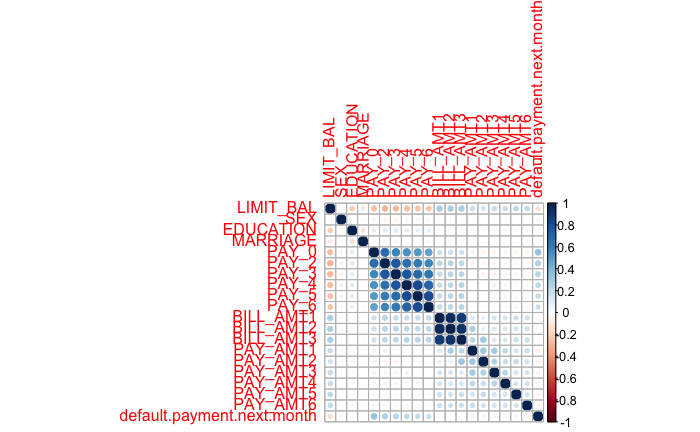
\includegraphics{q3_data_corr.png}
  \caption{Correlation analysis of the credit card default variables}
\end{figure}

The correlation between any of the variables is quite low, making the building of a robust model difficult.

\subsection{Statistical Model}

Our baseline BI model is build with all explanatory variable:
\begin{verbatim}
mbi <- gamlss(default.payment.next.month~LIMIT\_BAL+PAY\_0+PAY\_2+PAY\_3+PAY\_4+PAY\_5+PAY\_6+AGE+
                factor(EDUCATION)+factor(SEX)+factor(MARRIAGE)+BILL\_AMT1+PAY\_AMT1+BILL\_AMT2+PAY\_AMT2+
                BILL\_AMT3+PAY\_AMT3+BILL\_AMT4+PAY\_AMT4+BILL\_AMT5+PAY\_AMT5+BILL\_AMT6+PAY\_AMT6, 
              family=BI, # BI is for Binomial distribution
              data=cc\_train)
\end{verbatim}


\subsubsection{Selecting a Distribution}

The response variable \textbf{\texttt{default.payment.next.month}} is a binary value on the default event: one as 'Yes', zero as 'No'.
Binomial models are our only alternatives here. Manually fitting the different families show that the standard \textbf{Binomial Model}
\verb|BI| gives the best AIC scoring.  This is fortunate as with testing a large number of explanatory variable using stepwise
algorithms is already computationally expensive.


\subsection{Model Diagnostics}

\begin{figure}[H]
  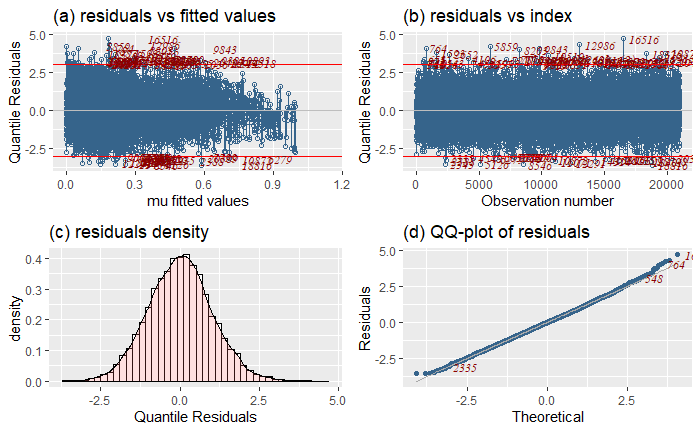
\includegraphics{q3_mbi_plot.png}
  \caption{BI residuals worm plot for credit card defaults}
\end{figure}

In this residuals analysis we start to see the problems before us.  The residuals worm plot has a high curvature and large extreme
values.

\begin{figure}[H]
  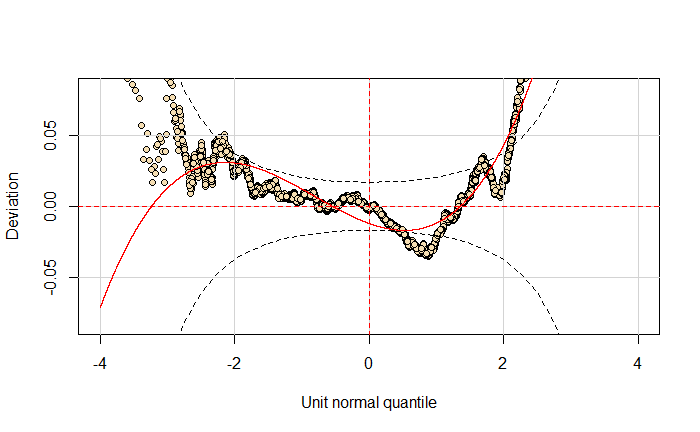
\includegraphics{q3_mbi_wp.png}
  \caption{BI residuals worm plot for credit card defaults}
\end{figure}

Using the \verb|stepGAICAll.B| function we find an improved AIC, but the worm plot is not much improved.

Using spline smoothing improves the situation markedly.

\begin{figure}[H]
  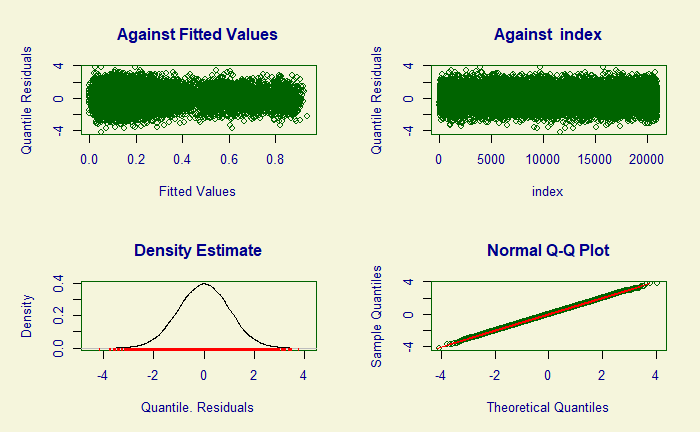
\includegraphics{q3_mbi4_plot.png}
  \caption{BI with smoothing and stepwise residuals plot}
\end{figure}

\begin{figure}[H]
  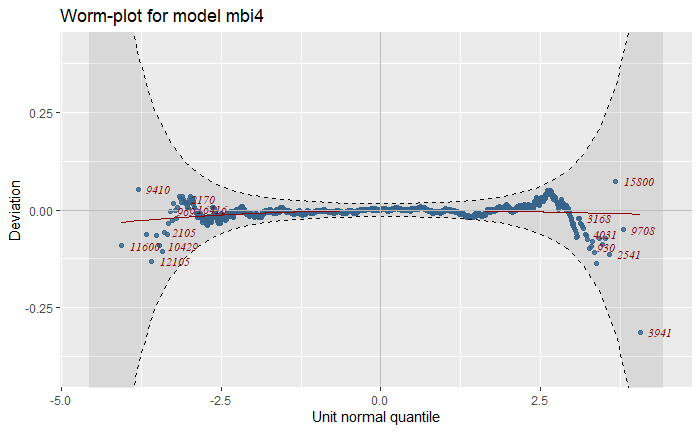
\includegraphics{q3_mbi4_wp.png}
  \caption{BI with smoothing and stepwise residuals worm plot}
\end{figure}



\subsection{Model Prediction}


\begin{verbatim}
library(pROC)
predicted_probabilities <- predict(mbi4, newdata = cc_validation, type = "response")
actual_values <- cc_validation$default.payment.next.month
roc_curve <- roc(cc_validation$default.payment.next.month, predicted_probabilities)
plot(roc_curve, main = "ROC Curve")


cor(predicted_probabilities, actual_values)
[1] 0.4489414
\end{verbatim}

\begin{figure}[H]
  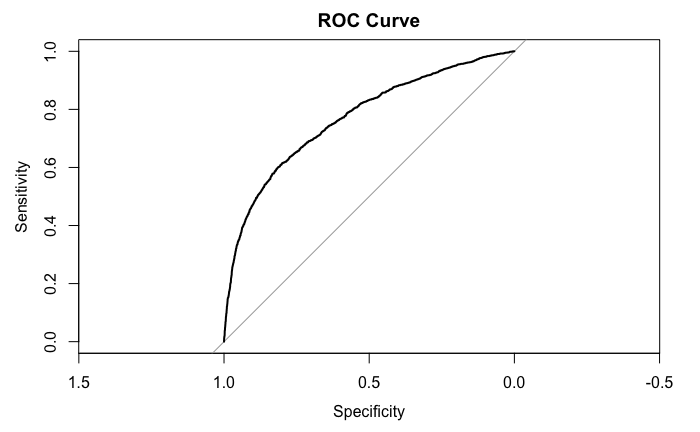
\includegraphics{q3_predict_roc.png}
  \caption{BI with smoothing and stepwise residuals worm plot}
\end{figure}

The correlation value is low.  This needs more work.


%\section{PeerReview}

(a) Choose one from a selection of student work on the third data set.

(b) Write a short critique on the adequacy of the work. You should look at:

\begin{itemize}
\item thequalityoftheexplorativeanalysisofthedataset
\item thechoiceofthedistributionfortheresponse(target)variable 
\item  themethodforselectingandcheckingthemodel
\item  theinterpretationoftheresults
\end{itemize}

(c) Give a grade [A, B, C, D, E, F] representing your estimation of the value of the work.



\pagebreak

\section{Conclusion}

\subsection{Summary of Findings}

Recap the key points discussed in the paper.

\subsection{Personal Insight}

Present your personal viewpoint developed through the research and implementation.


\subsection{Future Work}

Suggest areas for further research or potential improvements in the method.

\subsection{Final Thoughts}

Conclude with the significance of your findings for the field of cryptography.


\pagebreak

\printbibliography

\pagebreak

\appendix
\singlespacing

\section{Appendix A: R Code for Question 1}

To address the given task, we’ll go through it step by step, writing R code for each part. The task involves analyzing
BMI data for Dutch boys aged 15 to 16 years from the \texttt{dbbmi} dataset in the \texttt{gamlss.data} package, fitting
parametric distributions, and selecting an appropriate one based on the analysis.

First, let's load the data, subset it for the specific age group, and
plot the histogram to find a suitable value for \texttt{nbins}.

\section{Appendix A: R Code for Question 1}

To address the given task, we'll go through it step by step, writing R
code for each part. The task involves analyzing BMI data for Dutch boys
aged 10 to 11 years from the \texttt{dbbmi} dataset in the
\texttt{gamlss.data} package, fitting parametric distributions, and
selecting an appropriate one based on the analysis.

\hypertarget{instructions-on-how-to-analyse-the-first-data-set}{%
\subsection{Instructions on how to analyse the first data
set}\label{instructions-on-how-to-analyse-the-first-data-set}}

The first data set is a subset of Body Mass Index (BMI) data obtained
from the Fourth Dutch Growth Study, Fredriks et al.~2000 {[}1{]}. The
data contains BMI for different ages in years for Dutch boys. Each
student will be given a different age, for example, 10 to 11 years old.
The aim here is to find a suitable distribution of the BMI at this age.

\hypertarget{a-the-original-data-which-contains-all-ages-from-zero-to-twenty-two-exists-in-the-gamlss.data-package-under-the-name-of-dbbmi.-each-student-should-analyse-a-different-age.-here-we-give-an-example-how-to-analyse-age-10.-we-first-bring-the-data-set-in-r-and-then-create-a-subset-data.frame-containing-only-a-specific-age-here-from-10-11.-the-following-commands-can-be-used}{%
\subsubsection{(a) The original data, which contains all ages from zero
to twenty two, exists in the gamlss.data package under the name of
dbbmi. Each student should analyse a different age. Here we give an
example how to analyse age 10. We first bring the data set in R and then
create a subset data.frame containing only a specific age (here from
10-11). The following commands can be
used:}\label{a-the-original-data-which-contains-all-ages-from-zero-to-twenty-two-exists-in-the-gamlss.data-package-under-the-name-of-dbbmi.-each-student-should-analyse-a-different-age.-here-we-give-an-example-how-to-analyse-age-10.-we-first-bring-the-data-set-in-r-and-then-create-a-subset-data.frame-containing-only-a-specific-age-here-from-10-11.-the-following-commands-can-be-used}}

First, let's load the data, subset it for the specific age group, and
plot the histogram to find a suitable value for \texttt{nbins}.

\begin{Shaded}
\begin{Highlighting}[]
\CommentTok{\# suppress the warnings by setting warn={-}1 }
\FunctionTok{options}\NormalTok{(}\AttributeTok{warn=}\SpecialCharTok{{-}}\DecValTok{1}\NormalTok{) }

\CommentTok{\# Load the packages}
\FunctionTok{library}\NormalTok{(ggplot2)}
\FunctionTok{library}\NormalTok{(gamlss)}
\end{Highlighting}
\end{Shaded}

\begin{verbatim}
## Loading required package: splines
\end{verbatim}

\begin{verbatim}
## Loading required package: gamlss.data
\end{verbatim}

\begin{verbatim}
## 
## Attaching package: 'gamlss.data'
\end{verbatim}

\begin{verbatim}
## The following object is masked from 'package:datasets':
## 
##     sleep
\end{verbatim}

\begin{verbatim}
## Loading required package: gamlss.dist
\end{verbatim}

\begin{verbatim}
## Loading required package: nlme
\end{verbatim}

\begin{verbatim}
## Loading required package: parallel
\end{verbatim}

\begin{verbatim}
##  **********   GAMLSS Version 5.4-20  **********
\end{verbatim}

\begin{verbatim}
## For more on GAMLSS look at https://www.gamlss.com/
\end{verbatim}

\begin{verbatim}
## Type gamlssNews() to see new features/changes/bug fixes.
\end{verbatim}

\begin{Shaded}
\begin{Highlighting}[]
\FunctionTok{library}\NormalTok{(gamlss.ggplots)}
\end{Highlighting}
\end{Shaded}

\begin{verbatim}
## Loading required package: gamlss.foreach
\end{verbatim}

\begin{verbatim}
## Loading required package: foreach
\end{verbatim}

\begin{verbatim}
## Loading required package: doParallel
\end{verbatim}

\begin{verbatim}
## Loading required package: iterators
\end{verbatim}

\begin{Shaded}
\begin{Highlighting}[]
\FunctionTok{library}\NormalTok{(gamlss.add)}
\end{Highlighting}
\end{Shaded}

\begin{verbatim}
## Loading required package: mgcv
\end{verbatim}

\begin{verbatim}
## This is mgcv 1.9-0. For overview type 'help("mgcv-package")'.
\end{verbatim}

\begin{verbatim}
## Loading required package: nnet
\end{verbatim}

\begin{verbatim}
## 
## Attaching package: 'nnet'
\end{verbatim}

\begin{verbatim}
## The following object is masked from 'package:mgcv':
## 
##     multinom
\end{verbatim}

\begin{verbatim}
## Loading required package: rpart
\end{verbatim}

\begin{Shaded}
\begin{Highlighting}[]
\FunctionTok{library}\NormalTok{(gamlss.data)}
\FunctionTok{library}\NormalTok{(MASS)}

\CommentTok{\# Load the dataset}
\FunctionTok{data}\NormalTok{(dbbmi)}
\FunctionTok{summary}\NormalTok{(dbbmi)}
\end{Highlighting}
\end{Shaded}

\begin{verbatim}
##       age              bmi       
##  Min.   : 0.030   Min.   :11.17  
##  1st Qu.: 1.863   1st Qu.:15.96  
##  Median :10.450   Median :17.45  
##  Mean   : 9.291   Mean   :18.03  
##  3rd Qu.:15.130   3rd Qu.:19.60  
##  Max.   :21.700   Max.   :35.42
\end{verbatim}

\begin{Shaded}
\begin{Highlighting}[]
\CommentTok{\# Subset for ages 15 to 16}
\NormalTok{old }\OtherTok{\textless{}{-}} \DecValTok{15}
\NormalTok{dbbmi\_15 }\OtherTok{\textless{}{-}} \FunctionTok{with}\NormalTok{(dbbmi, }\FunctionTok{subset}\NormalTok{(dbbmi, age }\SpecialCharTok{\textgreater{}}\NormalTok{ old }\SpecialCharTok{\&}\NormalTok{ age }\SpecialCharTok{\textless{}}\NormalTok{ old }\SpecialCharTok{+} \DecValTok{1}\NormalTok{))}
\NormalTok{bmi15 }\OtherTok{\textless{}{-}}\NormalTok{ dbbmi\_15}\SpecialCharTok{$}\NormalTok{bmi}

\CommentTok{\# Plot the histogram; adjust nbins as needed to make the histogram look good}
\NormalTok{binwith }\OtherTok{=} \FloatTok{0.5}
\NormalTok{nbins }\OtherTok{=} \FunctionTok{trunc}\NormalTok{(}\FunctionTok{max}\NormalTok{(bmi15) }\SpecialCharTok{{-}} \FunctionTok{min}\NormalTok{(bmi15)) }\SpecialCharTok{/}\NormalTok{ binwith}

\FunctionTok{truehist}\NormalTok{(bmi15, }\AttributeTok{nbins=}\NormalTok{nbins)}
\end{Highlighting}
\end{Shaded}

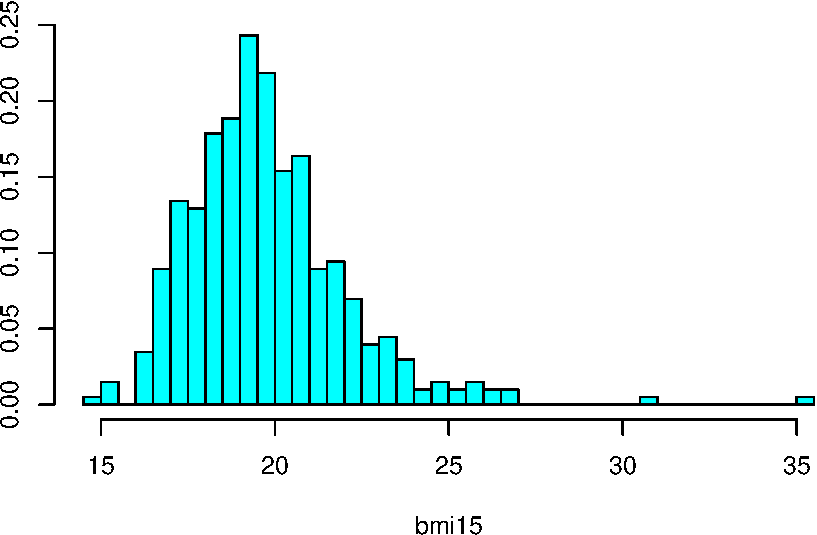
\includegraphics{assignment_q1_bmi_files/figure-latex/unnamed-chunk-1-1.pdf}

\begin{Shaded}
\begin{Highlighting}[]
\FunctionTok{density}\NormalTok{(bmi15, }\AttributeTok{cut =} \DecValTok{0}\NormalTok{)}
\end{Highlighting}
\end{Shaded}

\begin{verbatim}
## 
## Call:
##  density.default(x = bmi15, cut = 0)
## 
## Data: bmi15 (403 obs.);  Bandwidth 'bw' = 0.515
## 
##        x               y            
##  Min.   :14.70   Min.   :4.300e-07  
##  1st Qu.:19.78   1st Qu.:6.803e-04  
##  Median :24.87   Median :1.193e-02  
##  Mean   :24.87   Mean   :4.900e-02  
##  3rd Qu.:29.95   3rd Qu.:8.370e-02  
##  Max.   :35.03   Max.   :2.127e-01
\end{verbatim}

\begin{Shaded}
\begin{Highlighting}[]
\NormalTok{gamlss.ggplots}\SpecialCharTok{:::}\FunctionTok{y\_hist}\NormalTok{(dbbmi\_15}\SpecialCharTok{$}\NormalTok{bmi,}
                        \AttributeTok{from=}\FunctionTok{floor}\NormalTok{(}\FunctionTok{min}\NormalTok{(bmi15)), }
                        \AttributeTok{to=}\FunctionTok{ceiling}\NormalTok{(}\FunctionTok{max}\NormalTok{(bmi15)), }
                        \AttributeTok{binwidth=}\NormalTok{binwith,}
                        \AttributeTok{title=}\StringTok{"Histogram of BMI for 15 year olds"}\NormalTok{)}
\end{Highlighting}
\end{Shaded}

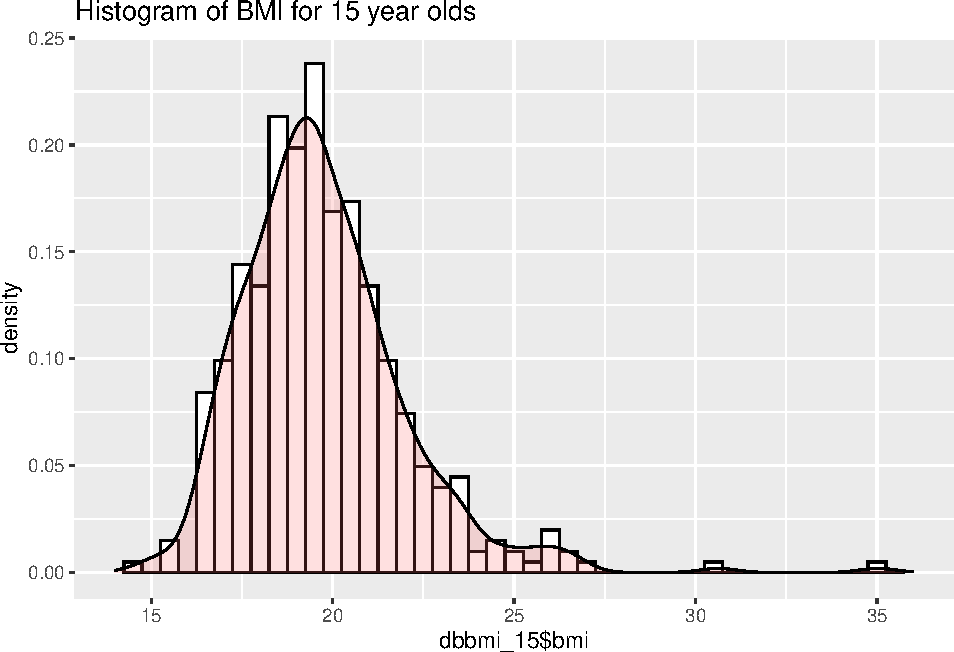
\includegraphics{assignment_q1_bmi_files/figure-latex/unnamed-chunk-1-2.pdf}

Experiment with the \texttt{nbins} parameter to find a visually
appealing and informative histogram. The goal is to have enough bins to
clearly see the distribution's shape without making it too noisy.

\hypertarget{b-fit-different-parametric-distributions-to-the-data-and-choose-an-appropriate-distribution-to-the-data.-justify-the-choice-of-the-distribution-by-explaining-what-you-have-done-and-why-you-select-this-specific-distribution.}{%
\subsubsection{(b) Fit different parametric distributions to the data
and choose an appropriate distribution to the data. Justify the choice
of the distribution by explaining what you have done and why you select
this specific
distribution.}\label{b-fit-different-parametric-distributions-to-the-data-and-choose-an-appropriate-distribution-to-the-data.-justify-the-choice-of-the-distribution-by-explaining-what-you-have-done-and-why-you-select-this-specific-distribution.}}

Next, we'll fit several parametric distributions to the data. Common
distributions for BMI data include the Normal, Log-Normal, and Gamma
distributions, among others. The \texttt{gamlss} package provides
functions to fit a wide range of distributions.

\begin{Shaded}
\begin{Highlighting}[]
\CommentTok{\# m1 is the model with the lowest AIC: list the best 6 fits:}
\CommentTok{\#m1 \textless{}{-} fitDist(bmi, type=c(\textquotesingle{}realplus\textquotesingle{}), data=dbbmi\_15, k=2)}
\CommentTok{\#m1$fit[1:6]}
\CommentTok{\#m1 \textless{}{-} fitDist(bmi, type=c(\textquotesingle{}realline\textquotesingle{}), data=dbbmi\_15, k=2)}
\CommentTok{\#m1$fit[1:6]}
\NormalTok{m1 }\OtherTok{\textless{}{-}} \FunctionTok{fitDist}\NormalTok{(bmi, }\AttributeTok{type=}\StringTok{\textquotesingle{}realAll\textquotesingle{}}\NormalTok{, }\AttributeTok{data=}\NormalTok{dbbmi\_15, }\AttributeTok{k=}\DecValTok{2}\NormalTok{)}
\end{Highlighting}
\end{Shaded}

\begin{verbatim}
##   |                                                                              |                                                                      |   0%  |                                                                              |=                                                                     |   2%  |                                                                              |===                                                                   |   4%  |                                                                              |====                                                                  |   6%  |                                                                              |=====                                                                 |   8%  |                                                                              |=======                                                               |  10%  |                                                                              |========                                                              |  12%  |                                                                              |==========                                                            |  14%  |                                                                              |===========                                                           |  16%  |                                                                              |============                                                          |  18%  |                                                                              |==============                                                        |  20%  |                                                                              |===============                                                       |  22%  |                                                                              |================                                                      |  24%  |                                                                              |==================                                                    |  25%  |                                                                              |===================                                                   |  27%  |                                                                              |=====================                                                 |  29%  |                                                                              |======================                                                |  31%  |                                                                              |=======================                                               |  33%  |                                                                              |=========================                                             |  35%  |                                                                              |==========================                                            |  37%  |                                                                              |===========================                                           |  39%  |                                                                              |=============================                                         |  41%  |                                                                              |==============================                                        |  43%  |                                                                              |================================                                      |  45%  |                                                                              |=================================                                     |  47%  |                                                                              |==================================                                    |  49%  |                                                                              |====================================                                  |  51%  |                                                                              |=====================================                                 |  53%  |                                                                              |======================================                                |  55%  |                                                                              |========================================                              |  57%  |                                                                              |=========================================                             |  59%  |                                                                              |===========================================                           |  61%  |                                                                              |============================================                          |  63%  |                                                                              |=============================================                         |  65%  |                                                                              |===============================================                       |  67%  |                                                                              |================================================                      |  69%  |                                                                              |=================================================                     |  71%  |                                                                              |===================================================                   |  73%  |                                                                              |====================================================                  |  75%  |                                                                              |======================================================                |  76%  |                                                                              |=======================================================               |  78%  |                                                                              |========================================================              |  80%  |                                                                              |==========================================================            |  82%  |                                                                              |===========================================================           |  84%  |                                                                              |============================================================          |  86%  |                                                                              |==============================================================        |  88%  |                                                                              |===============================================================       |  90%  |                                                                              |=================================================================     |  92%  |                                                                              |==================================================================    |  94%  |                                                                              |===================================================================   |  96%  |                                                                              |===================================================================== |  98%  |                                                                              |======================================================================| 100%
\end{verbatim}

\begin{Shaded}
\begin{Highlighting}[]
\NormalTok{m1}\SpecialCharTok{$}\NormalTok{fit[}\DecValTok{1}\SpecialCharTok{:}\DecValTok{6}\NormalTok{]}
\end{Highlighting}
\end{Shaded}

\begin{verbatim}
##   exGAUS    BCPEo     BCPE     BCTo      BCT      ST5 
## 1729.537 1729.731 1729.731 1729.992 1729.992 1730.401
\end{verbatim}

\begin{Shaded}
\begin{Highlighting}[]
\NormalTok{m1 }\OtherTok{\textless{}{-}} \FunctionTok{histDist}\NormalTok{(bmi, }\StringTok{"exGAUS"}\NormalTok{, }\AttributeTok{density=}\ConstantTok{TRUE}\NormalTok{, }\AttributeTok{line.col=}\FunctionTok{c}\NormalTok{(}\DecValTok{1}\NormalTok{,}\DecValTok{1}\NormalTok{), }\AttributeTok{line.ty=}\FunctionTok{c}\NormalTok{(}\DecValTok{1}\NormalTok{,}\DecValTok{2}\NormalTok{), }\AttributeTok{nbins=}\NormalTok{nbins, }\AttributeTok{data=}\NormalTok{dbbmi\_15)}
\end{Highlighting}
\end{Shaded}

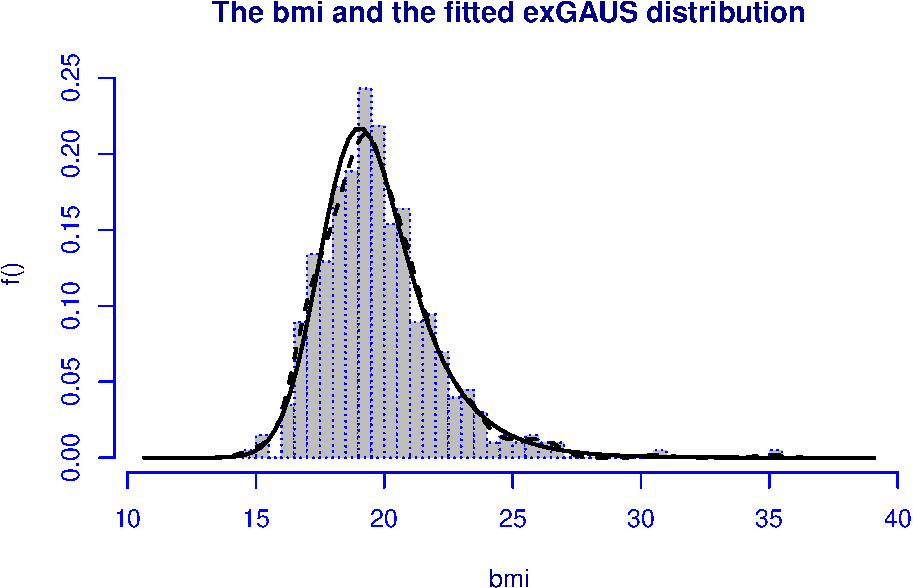
\includegraphics{assignment_q1_bmi_files/figure-latex/unnamed-chunk-3-1.pdf}

\begin{Shaded}
\begin{Highlighting}[]
\FunctionTok{plot}\NormalTok{(m1)}
\end{Highlighting}
\end{Shaded}

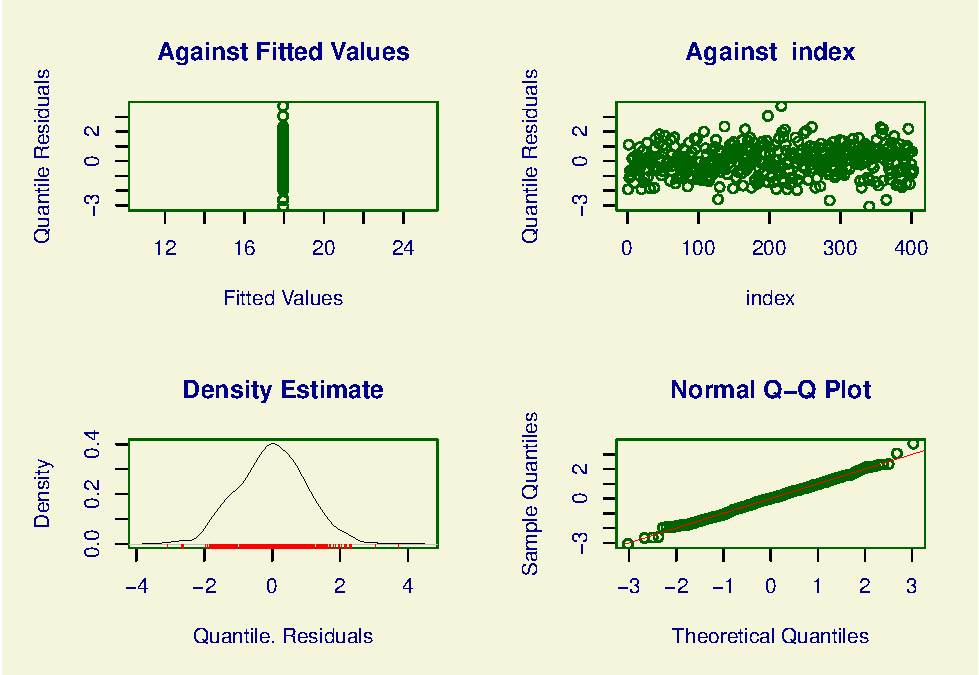
\includegraphics{assignment_q1_bmi_files/figure-latex/unnamed-chunk-3-2.pdf}

\begin{verbatim}
## ******************************************************************
##        Summary of the Quantile Residuals
##                            mean   =  -0.00222054 
##                        variance   =  1.005728 
##                coef. of skewness  =  0.05915047 
##                coef. of kurtosis  =  3.193805 
## Filliben correlation coefficient  =  0.9982076 
## ******************************************************************
\end{verbatim}

\begin{Shaded}
\begin{Highlighting}[]
\NormalTok{m2 }\OtherTok{\textless{}{-}} \FunctionTok{histDist}\NormalTok{(bmi, }\StringTok{"BCPEo"}\NormalTok{, }\AttributeTok{density=}\ConstantTok{TRUE}\NormalTok{, }\AttributeTok{line.col=}\FunctionTok{c}\NormalTok{(}\DecValTok{1}\NormalTok{,}\DecValTok{1}\NormalTok{), }\AttributeTok{line.ty=}\FunctionTok{c}\NormalTok{(}\DecValTok{1}\NormalTok{,}\DecValTok{2}\NormalTok{), }\AttributeTok{nbins=}\NormalTok{nbins, }\AttributeTok{data=}\NormalTok{dbbmi\_15)}
\end{Highlighting}
\end{Shaded}

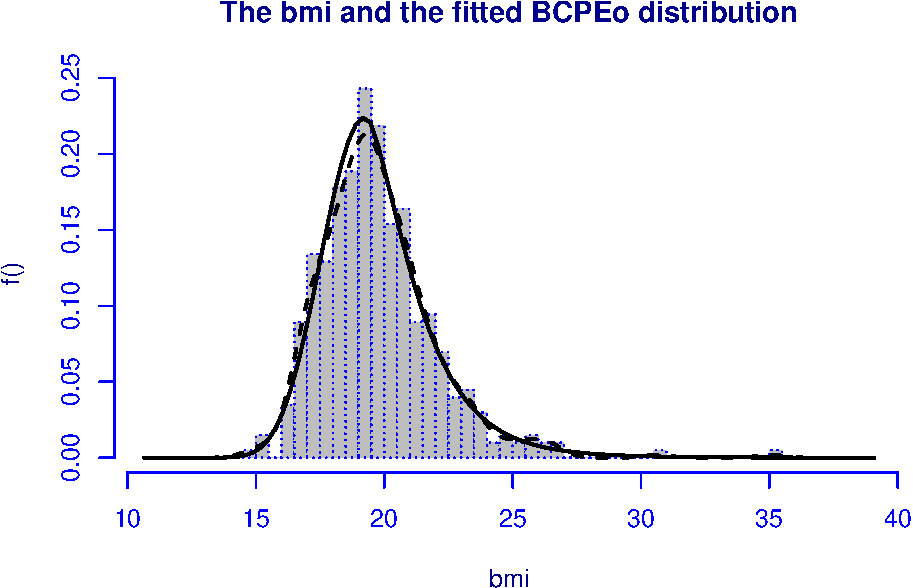
\includegraphics{assignment_q1_bmi_files/figure-latex/unnamed-chunk-3-3.pdf}

\begin{Shaded}
\begin{Highlighting}[]
\FunctionTok{plot}\NormalTok{(m2)}
\end{Highlighting}
\end{Shaded}

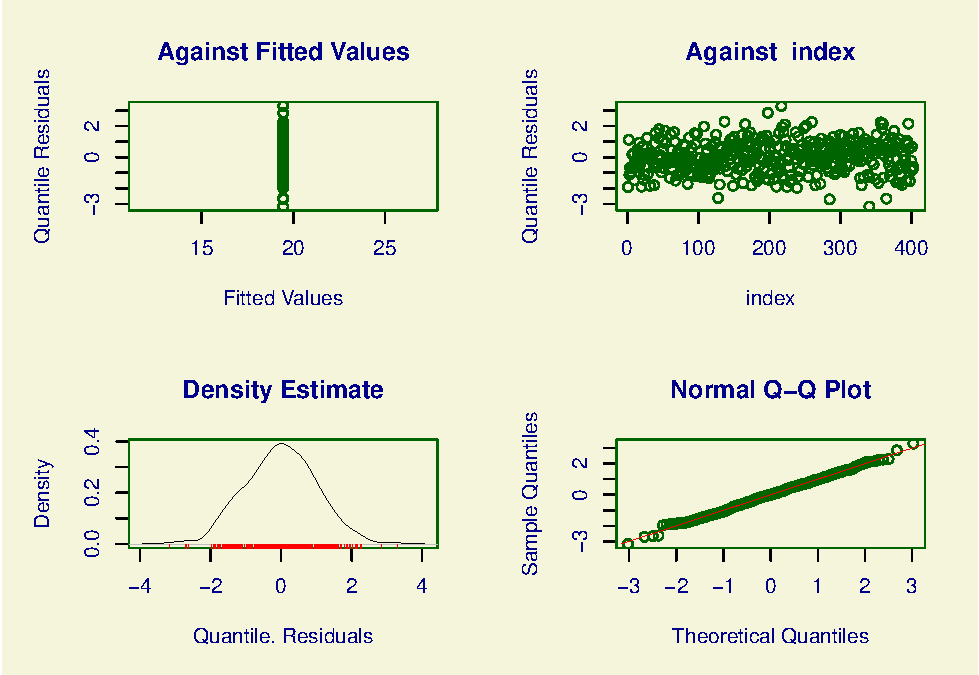
\includegraphics{assignment_q1_bmi_files/figure-latex/unnamed-chunk-3-4.pdf}

\begin{verbatim}
## ******************************************************************
##        Summary of the Quantile Residuals
##                            mean   =  -0.002539429 
##                        variance   =  1.00257 
##                coef. of skewness  =  -0.001697173 
##                coef. of kurtosis  =  2.997353 
## Filliben correlation coefficient  =  0.9988481 
## ******************************************************************
\end{verbatim}

\begin{Shaded}
\begin{Highlighting}[]
\NormalTok{m3 }\OtherTok{\textless{}{-}} \FunctionTok{histDist}\NormalTok{(bmi, }\StringTok{"BCPE"}\NormalTok{, }\AttributeTok{density=}\ConstantTok{TRUE}\NormalTok{, }\AttributeTok{line.col=}\FunctionTok{c}\NormalTok{(}\DecValTok{1}\NormalTok{,}\DecValTok{1}\NormalTok{), }\AttributeTok{line.ty=}\FunctionTok{c}\NormalTok{(}\DecValTok{1}\NormalTok{,}\DecValTok{2}\NormalTok{), }\AttributeTok{nbins=}\NormalTok{nbins, }\AttributeTok{data=}\NormalTok{dbbmi\_15)}
\end{Highlighting}
\end{Shaded}

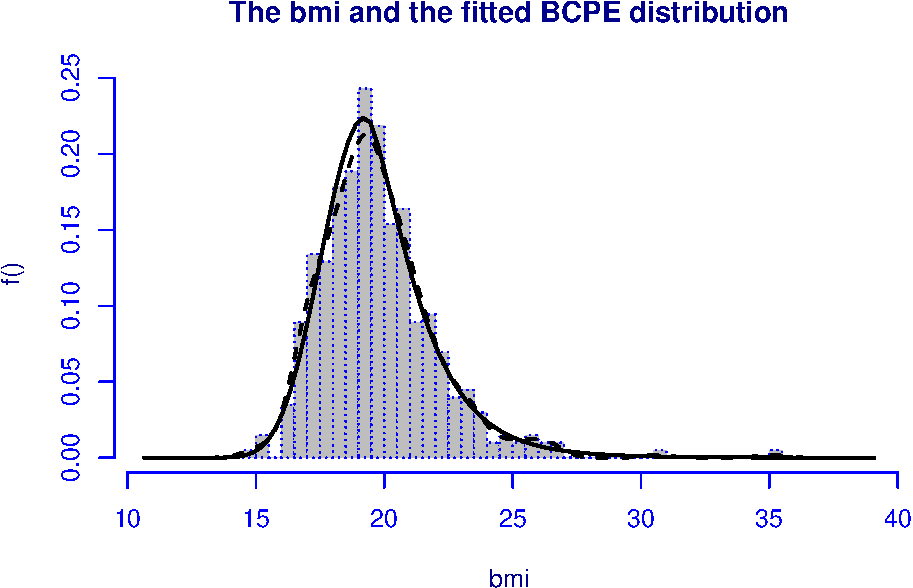
\includegraphics{assignment_q1_bmi_files/figure-latex/unnamed-chunk-3-5.pdf}

\begin{Shaded}
\begin{Highlighting}[]
\FunctionTok{plot}\NormalTok{(m3)}
\end{Highlighting}
\end{Shaded}

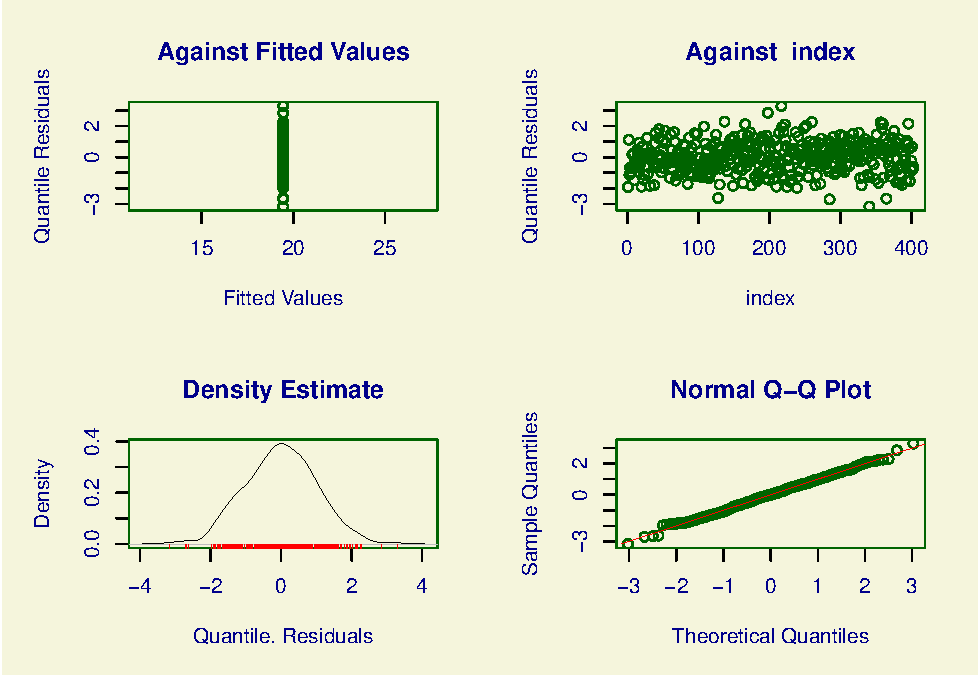
\includegraphics{assignment_q1_bmi_files/figure-latex/unnamed-chunk-3-6.pdf}

\begin{verbatim}
## ******************************************************************
##        Summary of the Quantile Residuals
##                            mean   =  -0.002537045 
##                        variance   =  1.00257 
##                coef. of skewness  =  -0.001697852 
##                coef. of kurtosis  =  2.997391 
## Filliben correlation coefficient  =  0.9988481 
## ******************************************************************
\end{verbatim}

\begin{Shaded}
\begin{Highlighting}[]
\NormalTok{m1 }\OtherTok{\textless{}{-}} \FunctionTok{gamlss}\NormalTok{(bmi}\SpecialCharTok{\textasciitilde{}}\DecValTok{1}\NormalTok{, }\AttributeTok{family=}\NormalTok{NO, }\AttributeTok{data=}\NormalTok{dbbmi\_15)}
\end{Highlighting}
\end{Shaded}

\begin{verbatim}
## GAMLSS-RS iteration 1: Global Deviance = 1803.044 
## GAMLSS-RS iteration 2: Global Deviance = 1803.044
\end{verbatim}

\begin{Shaded}
\begin{Highlighting}[]
\NormalTok{c1 }\OtherTok{\textless{}{-}} \FunctionTok{chooseDist}\NormalTok{(m1, }\AttributeTok{type=}\StringTok{\textquotesingle{}realAll\textquotesingle{}}\NormalTok{, }\AttributeTok{data=}\NormalTok{dbbmi\_15, }\AttributeTok{parallel=}\StringTok{"snow"}\NormalTok{, }\AttributeTok{ncpus=}\DecValTok{4}\NormalTok{)}
\end{Highlighting}
\end{Shaded}

\begin{verbatim}
## minimum GAIC(k= 2 ) family: exGAUS 
## minimum GAIC(k= 3.84 ) family: exGAUS 
## minimum GAIC(k= 6 ) family: exGAUS
\end{verbatim}

\begin{Shaded}
\begin{Highlighting}[]
\NormalTok{c1}
\end{Highlighting}
\end{Shaded}

\begin{verbatim}
##                 2     3.84        6
## NO       1807.044 1810.724 1815.044
## GU       2117.531 2121.211 2125.531
## RG       1733.816 1737.496 1741.816
## LO       1761.949 1765.629 1769.949
## NET      1759.479 1763.159 1767.479
## TF       1756.536 1762.056 1768.536
## TF2      1756.537 1762.057 1768.537
## PE       1766.779 1772.299 1778.779
## PE2      1766.783 1772.303 1778.783
## SN1      1809.044 1814.564 1821.044
## SN2      1755.128 1760.648 1767.128
## exGAUS   1729.537 1735.057 1741.537
## SHASH    1735.278 1742.638 1751.278
## SHASHo   1740.368 1747.728 1756.368
## SHASHo2  1740.098 1747.458 1756.098
## EGB2     1734.237 1741.597 1750.237
## JSU      1731.709 1739.069 1747.709
## JSUo     1739.039 1746.399 1755.039
## SEP1     1742.582 1749.942 1758.582
## SEP2     1749.584 1756.944 1765.584
## SEP3     1742.365 1749.725 1758.365
## SEP4     1732.778 1740.138 1748.778
## ST1      1734.015 1741.375 1750.015
## ST2      1737.021 1744.381 1753.021
## ST3      1735.795 1743.155 1751.795
## ST4      1733.081 1740.441 1749.081
## ST5      1732.808 1740.168 1748.808
## SST      1735.770 1743.130 1751.770
## GT       1757.541 1764.901 1773.541
## EXP      3212.376 3214.216 3216.376
## GA       1772.064 1775.744 1780.064
## IG       1759.441 1763.121 1767.441
## LOGNO    1758.605 1762.285 1766.605
## LOGNO2   1758.605 1762.285 1766.605
## WEI      1966.621 1970.301 1974.621
## WEI2     2373.622 2377.302 2381.622
## WEI3     1966.621 1970.301 1974.621
## IGAMMA   1748.193 1751.873 1756.193
## PARETO2  3251.903 3255.583 3259.903
## PARETO2o 3222.313 3225.993 3230.313
## GP       3251.903 3255.583 3259.903
## BCCG     1730.663 1736.183 1742.663
## BCCGo    1730.663 1736.183 1742.663
## GG       1732.317 1737.837 1744.317
## GIG      1750.193 1755.713 1762.193
## LNO      1758.605 1762.285 1766.605
## BCTo     1729.992 1737.352 1745.992
## BCT      1729.992 1737.352 1745.992
## BCPEo    1729.731 1737.091 1745.731
## BCPE     1729.731 1737.091 1745.731
## GB2      1732.204 1739.564 1748.204
\end{verbatim}

\hypertarget{best-fit-is-bccg}{%
\paragraph{Best fit is BCCG}\label{best-fit-is-bccg}}

\begin{Shaded}
\begin{Highlighting}[]
\CommentTok{\# Best fit is BCCG}
\NormalTok{m1 }\OtherTok{\textless{}{-}} \FunctionTok{histDist}\NormalTok{(bmi, }\StringTok{"BCCG"}\NormalTok{, }\AttributeTok{density=}\ConstantTok{TRUE}\NormalTok{, }\AttributeTok{line.col=}\FunctionTok{c}\NormalTok{(}\DecValTok{1}\NormalTok{,}\DecValTok{1}\NormalTok{), }\AttributeTok{line.ty=}\FunctionTok{c}\NormalTok{(}\DecValTok{1}\NormalTok{,}\DecValTok{2}\NormalTok{), }\AttributeTok{nbins=}\NormalTok{nbins, }\AttributeTok{data=}\NormalTok{dbbmi\_15)}
\end{Highlighting}
\end{Shaded}

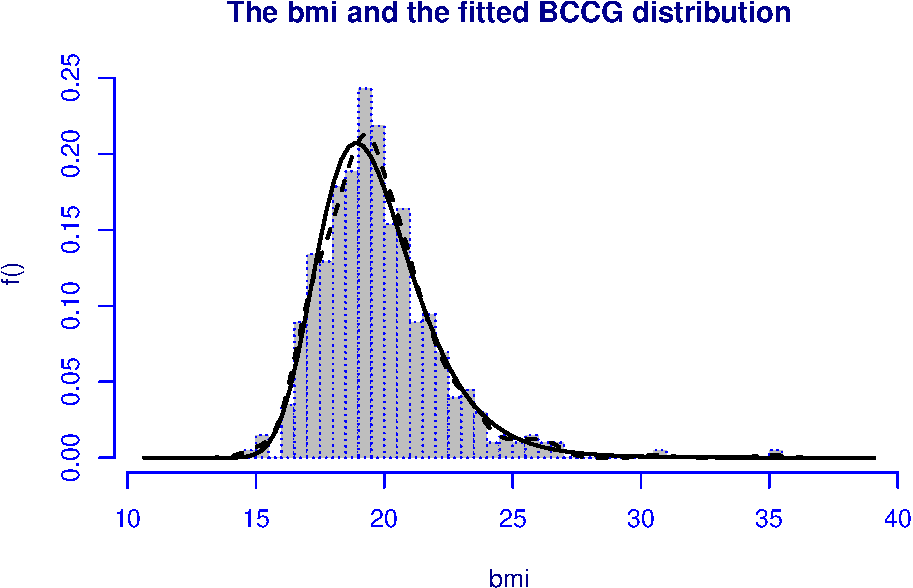
\includegraphics{assignment_q1_bmi_files/figure-latex/unnamed-chunk-5-1.pdf}

\begin{Shaded}
\begin{Highlighting}[]
\FunctionTok{plot}\NormalTok{(m1)}
\end{Highlighting}
\end{Shaded}

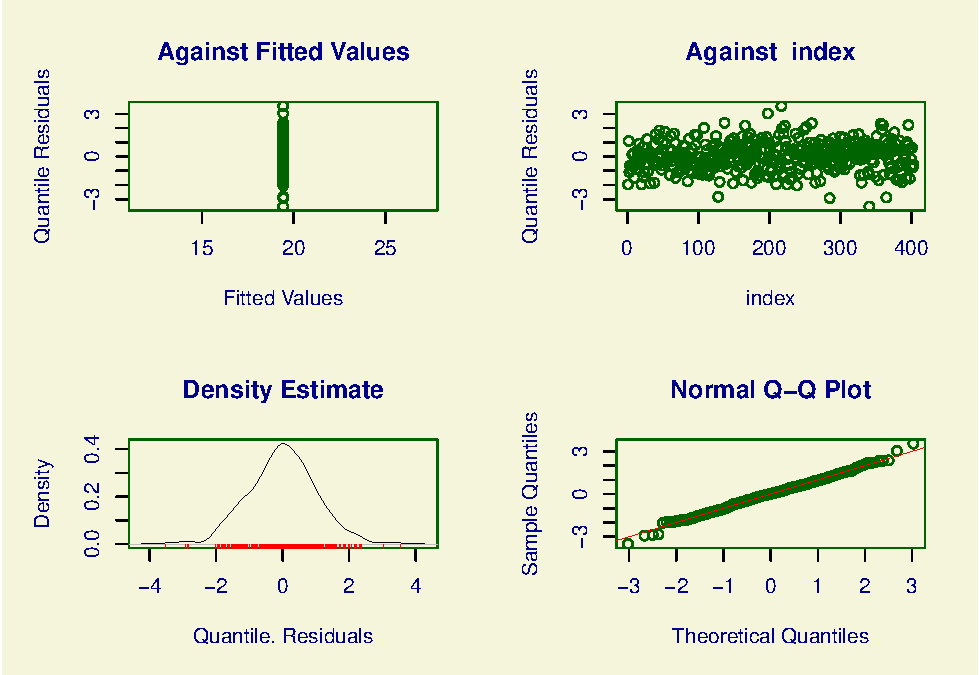
\includegraphics{assignment_q1_bmi_files/figure-latex/unnamed-chunk-5-2.pdf}

\begin{verbatim}
## ******************************************************************
##        Summary of the Quantile Residuals
##                            mean   =  1.683958e-07 
##                        variance   =  1.002488 
##                coef. of skewness  =  -0.0312982 
##                coef. of kurtosis  =  3.44508 
## Filliben correlation coefficient  =  0.9976684 
## ******************************************************************
\end{verbatim}

\begin{Shaded}
\begin{Highlighting}[]
\NormalTok{m2 }\OtherTok{\textless{}{-}} \FunctionTok{histDist}\NormalTok{(bmi, }\StringTok{"TF"}\NormalTok{, }\AttributeTok{density=}\ConstantTok{TRUE}\NormalTok{, }\AttributeTok{line.col=}\FunctionTok{c}\NormalTok{(}\DecValTok{1}\NormalTok{,}\DecValTok{1}\NormalTok{), }\AttributeTok{line.ty=}\FunctionTok{c}\NormalTok{(}\DecValTok{1}\NormalTok{,}\DecValTok{2}\NormalTok{), }\AttributeTok{nbins=}\NormalTok{nbins, }\AttributeTok{data=}\NormalTok{dbbmi\_15)}
\end{Highlighting}
\end{Shaded}

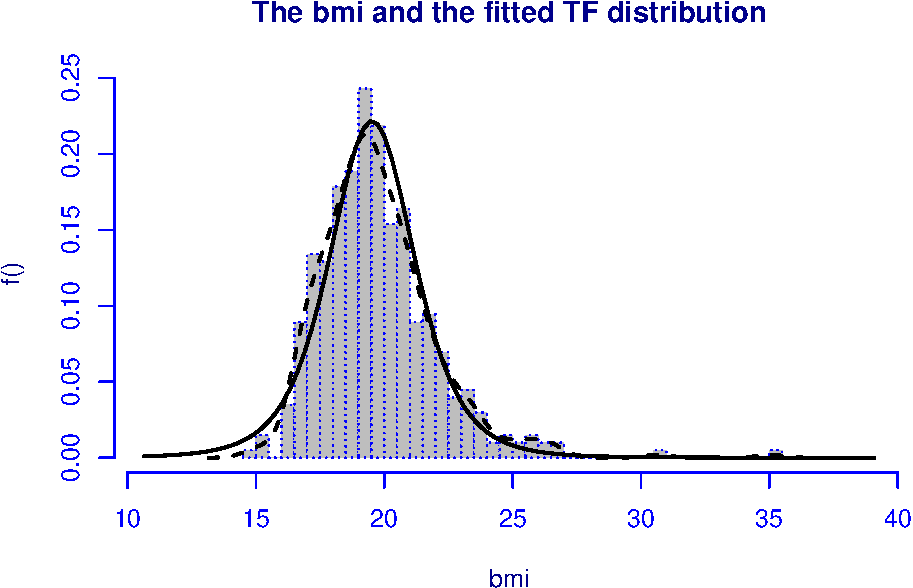
\includegraphics{assignment_q1_bmi_files/figure-latex/unnamed-chunk-5-3.pdf}

\begin{Shaded}
\begin{Highlighting}[]
\FunctionTok{plot}\NormalTok{(m2)}
\end{Highlighting}
\end{Shaded}

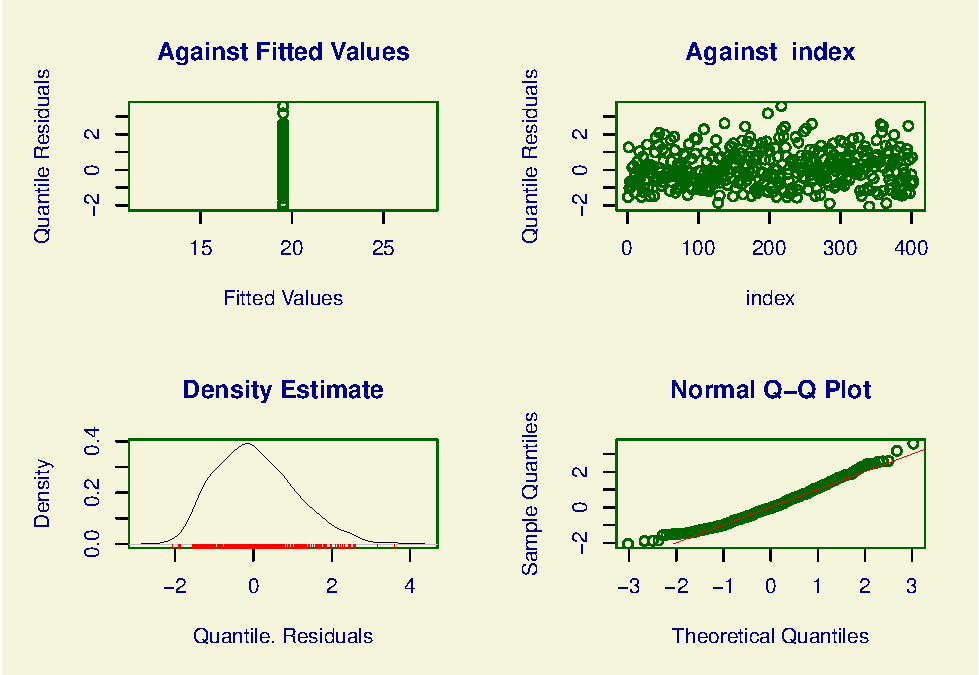
\includegraphics{assignment_q1_bmi_files/figure-latex/unnamed-chunk-5-4.pdf}

\begin{verbatim}
## ******************************************************************
##        Summary of the Quantile Residuals
##                            mean   =  0.06736512 
##                        variance   =  0.9980666 
##                coef. of skewness  =  0.4946411 
##                coef. of kurtosis  =  2.93465 
## Filliben correlation coefficient  =  0.990266 
## ******************************************************************
\end{verbatim}

\begin{Shaded}
\begin{Highlighting}[]
\NormalTok{m3 }\OtherTok{\textless{}{-}} \FunctionTok{histDist}\NormalTok{(bmi, }\StringTok{"exGAUS"}\NormalTok{, }\AttributeTok{density=}\ConstantTok{TRUE}\NormalTok{, }\AttributeTok{line.col=}\FunctionTok{c}\NormalTok{(}\DecValTok{1}\NormalTok{,}\DecValTok{1}\NormalTok{), }\AttributeTok{line.ty=}\FunctionTok{c}\NormalTok{(}\DecValTok{1}\NormalTok{,}\DecValTok{2}\NormalTok{), }\AttributeTok{nbins=}\NormalTok{nbins, }\AttributeTok{data=}\NormalTok{dbbmi\_15)}
\end{Highlighting}
\end{Shaded}

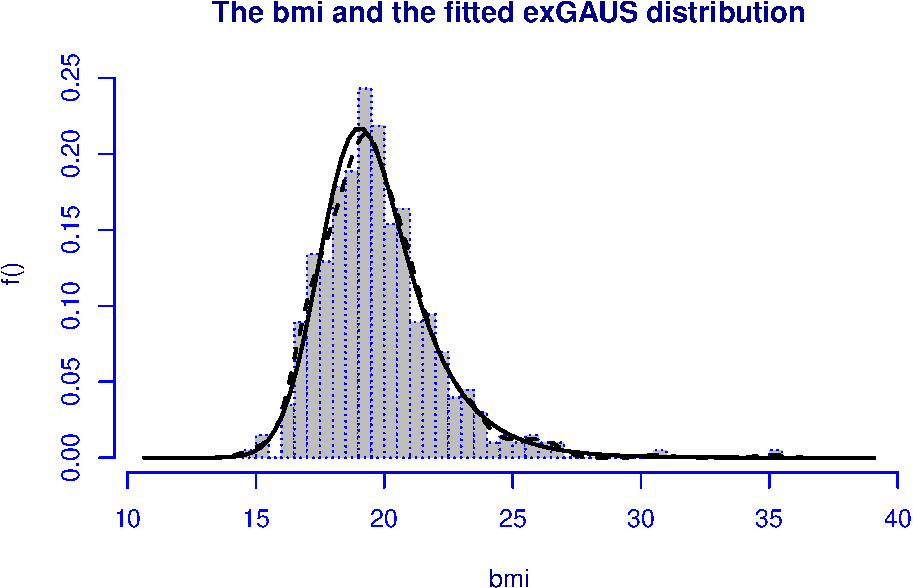
\includegraphics{assignment_q1_bmi_files/figure-latex/unnamed-chunk-5-5.pdf}

\begin{Shaded}
\begin{Highlighting}[]
\FunctionTok{plot}\NormalTok{(m3)}
\end{Highlighting}
\end{Shaded}

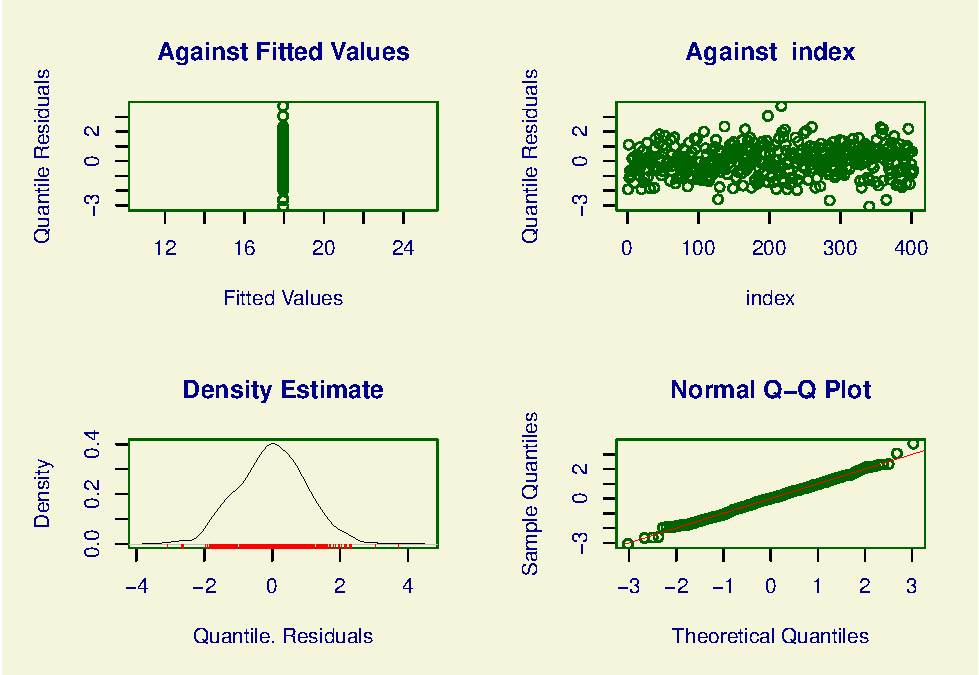
\includegraphics{assignment_q1_bmi_files/figure-latex/unnamed-chunk-5-6.pdf}

\begin{verbatim}
## ******************************************************************
##        Summary of the Quantile Residuals
##                            mean   =  -0.00222054 
##                        variance   =  1.005728 
##                coef. of skewness  =  0.05915047 
##                coef. of kurtosis  =  3.193805 
## Filliben correlation coefficient  =  0.9982076 
## ******************************************************************
\end{verbatim}

\begin{Shaded}
\begin{Highlighting}[]
\FunctionTok{plot}\NormalTok{(}\ControlFlowTok{function}\NormalTok{(x) }\FunctionTok{dJSU}\NormalTok{(x, }\AttributeTok{mu=}\FloatTok{16.8475}\NormalTok{, }\AttributeTok{sigma=}\FloatTok{1.7560}\NormalTok{, }\AttributeTok{nu=}\FloatTok{2.439}\NormalTok{, }\AttributeTok{tau=}\FloatTok{2.6890}\NormalTok{), }\DecValTok{10}\NormalTok{, }\DecValTok{25}\NormalTok{, }\AttributeTok{main =} \StringTok{"The JSU  density mu=16.8475, sigma=0.7560, nu=2.439, tau=0.6890"}\NormalTok{)}
\end{Highlighting}
\end{Shaded}

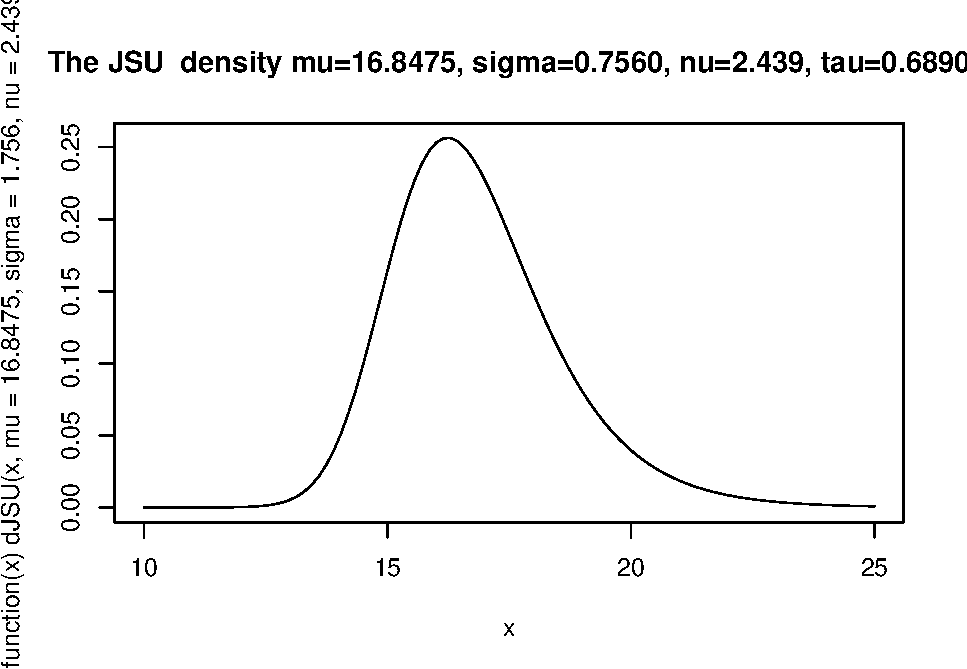
\includegraphics{assignment_q1_bmi_files/figure-latex/unnamed-chunk-6-1.pdf}

\begin{Shaded}
\begin{Highlighting}[]
\CommentTok{\#print(dJSU(x, mu=16.8475, sigma=1.7560, nu=2.439, tau=2.742))}
\end{Highlighting}
\end{Shaded}

\begin{Shaded}
\begin{Highlighting}[]
\CommentTok{\# Fit different distributions}
\NormalTok{fit\_bccg }\OtherTok{\textless{}{-}} \FunctionTok{gamlss}\NormalTok{(bmi15 }\SpecialCharTok{\textasciitilde{}} \DecValTok{1}\NormalTok{, }\AttributeTok{family=}\NormalTok{BCCG)}
\end{Highlighting}
\end{Shaded}

\begin{verbatim}
## GAMLSS-RS iteration 1: Global Deviance = 1732.959 
## GAMLSS-RS iteration 2: Global Deviance = 1725.178 
## GAMLSS-RS iteration 3: Global Deviance = 1724.682 
## GAMLSS-RS iteration 4: Global Deviance = 1724.664 
## GAMLSS-RS iteration 5: Global Deviance = 1724.663
\end{verbatim}

\begin{Shaded}
\begin{Highlighting}[]
\NormalTok{fit\_jsu }\OtherTok{\textless{}{-}} \FunctionTok{gamlss}\NormalTok{(bmi15 }\SpecialCharTok{\textasciitilde{}} \DecValTok{1}\NormalTok{, }\AttributeTok{family=}\NormalTok{JSU)}
\end{Highlighting}
\end{Shaded}

\begin{verbatim}
## GAMLSS-RS iteration 1: Global Deviance = 1759.315 
## GAMLSS-RS iteration 2: Global Deviance = 1741.358 
## GAMLSS-RS iteration 3: Global Deviance = 1733.024 
## GAMLSS-RS iteration 4: Global Deviance = 1728.984 
## GAMLSS-RS iteration 5: Global Deviance = 1726.744 
## GAMLSS-RS iteration 6: Global Deviance = 1725.473 
## GAMLSS-RS iteration 7: Global Deviance = 1724.745 
## GAMLSS-RS iteration 8: Global Deviance = 1724.328 
## GAMLSS-RS iteration 9: Global Deviance = 1724.085 
## GAMLSS-RS iteration 10: Global Deviance = 1723.94 
## GAMLSS-RS iteration 11: Global Deviance = 1723.855 
## GAMLSS-RS iteration 12: Global Deviance = 1723.801 
## GAMLSS-RS iteration 13: Global Deviance = 1723.767 
## GAMLSS-RS iteration 14: Global Deviance = 1723.746 
## GAMLSS-RS iteration 15: Global Deviance = 1723.732 
## GAMLSS-RS iteration 16: Global Deviance = 1723.723 
## GAMLSS-RS iteration 17: Global Deviance = 1723.717 
## GAMLSS-RS iteration 18: Global Deviance = 1723.713 
## GAMLSS-RS iteration 19: Global Deviance = 1723.711 
## GAMLSS-RS iteration 20: Global Deviance = 1723.709
\end{verbatim}

\begin{Shaded}
\begin{Highlighting}[]
\NormalTok{fit\_tf }\OtherTok{\textless{}{-}} \FunctionTok{gamlss}\NormalTok{(bmi15 }\SpecialCharTok{\textasciitilde{}} \DecValTok{1}\NormalTok{, }\AttributeTok{family=}\NormalTok{TF)}
\end{Highlighting}
\end{Shaded}

\begin{verbatim}
## GAMLSS-RS iteration 1: Global Deviance = 1754.007 
## GAMLSS-RS iteration 2: Global Deviance = 1751.186 
## GAMLSS-RS iteration 3: Global Deviance = 1750.66 
## GAMLSS-RS iteration 4: Global Deviance = 1750.56 
## GAMLSS-RS iteration 5: Global Deviance = 1750.541 
## GAMLSS-RS iteration 6: Global Deviance = 1750.537 
## GAMLSS-RS iteration 7: Global Deviance = 1750.536
\end{verbatim}

\begin{Shaded}
\begin{Highlighting}[]
\NormalTok{fit\_lognorm }\OtherTok{\textless{}{-}} \FunctionTok{gamlss}\NormalTok{(bmi15 }\SpecialCharTok{\textasciitilde{}} \DecValTok{1}\NormalTok{, }\AttributeTok{family=}\NormalTok{LOGNO)}
\end{Highlighting}
\end{Shaded}

\begin{verbatim}
## GAMLSS-RS iteration 1: Global Deviance = 1754.605 
## GAMLSS-RS iteration 2: Global Deviance = 1754.605
\end{verbatim}

\begin{Shaded}
\begin{Highlighting}[]
\NormalTok{fit\_lo }\OtherTok{\textless{}{-}} \FunctionTok{gamlss}\NormalTok{(bmi15 }\SpecialCharTok{\textasciitilde{}} \DecValTok{1}\NormalTok{, }\AttributeTok{family=}\NormalTok{LO)}
\end{Highlighting}
\end{Shaded}

\begin{verbatim}
## GAMLSS-RS iteration 1: Global Deviance = 1758.388 
## GAMLSS-RS iteration 2: Global Deviance = 1757.949 
## GAMLSS-RS iteration 3: Global Deviance = 1757.949
\end{verbatim}

\begin{Shaded}
\begin{Highlighting}[]
\NormalTok{fit\_pe }\OtherTok{\textless{}{-}} \FunctionTok{gamlss}\NormalTok{(bmi15 }\SpecialCharTok{\textasciitilde{}} \DecValTok{1}\NormalTok{, }\AttributeTok{family=}\NormalTok{PE)}
\end{Highlighting}
\end{Shaded}

\begin{verbatim}
## GAMLSS-RS iteration 1: Global Deviance = 1761.569 
## GAMLSS-RS iteration 2: Global Deviance = 1760.787 
## GAMLSS-RS iteration 3: Global Deviance = 1760.779 
## GAMLSS-RS iteration 4: Global Deviance = 1760.779
\end{verbatim}

\begin{Shaded}
\begin{Highlighting}[]
\NormalTok{fit\_gamma }\OtherTok{\textless{}{-}} \FunctionTok{gamlss}\NormalTok{(bmi15 }\SpecialCharTok{\textasciitilde{}} \DecValTok{1}\NormalTok{, }\AttributeTok{family=}\NormalTok{GA)}
\end{Highlighting}
\end{Shaded}

\begin{verbatim}
## GAMLSS-RS iteration 1: Global Deviance = 1768.064 
## GAMLSS-RS iteration 2: Global Deviance = 1768.064
\end{verbatim}

\begin{Shaded}
\begin{Highlighting}[]
\NormalTok{fit\_norm }\OtherTok{\textless{}{-}} \FunctionTok{gamlss}\NormalTok{(bmi15 }\SpecialCharTok{\textasciitilde{}} \DecValTok{1}\NormalTok{, }\AttributeTok{family=}\NormalTok{NO)}
\end{Highlighting}
\end{Shaded}

\begin{verbatim}
## GAMLSS-RS iteration 1: Global Deviance = 1803.044 
## GAMLSS-RS iteration 2: Global Deviance = 1803.044
\end{verbatim}

\begin{Shaded}
\begin{Highlighting}[]
\NormalTok{fit\_wei }\OtherTok{\textless{}{-}} \FunctionTok{gamlss}\NormalTok{(bmi15 }\SpecialCharTok{\textasciitilde{}} \DecValTok{1}\NormalTok{, }\AttributeTok{family=}\NormalTok{WEI)}
\end{Highlighting}
\end{Shaded}

\begin{verbatim}
## GAMLSS-RS iteration 1: Global Deviance = 2065.919 
## GAMLSS-RS iteration 2: Global Deviance = 1962.633 
## GAMLSS-RS iteration 3: Global Deviance = 1962.621 
## GAMLSS-RS iteration 4: Global Deviance = 1962.621
\end{verbatim}

\begin{Shaded}
\begin{Highlighting}[]
\NormalTok{fit\_gu }\OtherTok{\textless{}{-}} \FunctionTok{gamlss}\NormalTok{(bmi15 }\SpecialCharTok{\textasciitilde{}} \DecValTok{1}\NormalTok{, }\AttributeTok{family=}\NormalTok{GU)}
\end{Highlighting}
\end{Shaded}

\begin{verbatim}
## GAMLSS-RS iteration 1: Global Deviance = 2430.46 
## GAMLSS-RS iteration 2: Global Deviance = 2115.898 
## GAMLSS-RS iteration 3: Global Deviance = 2113.566 
## GAMLSS-RS iteration 4: Global Deviance = 2113.537 
## GAMLSS-RS iteration 5: Global Deviance = 2113.534 
## GAMLSS-RS iteration 6: Global Deviance = 2113.533 
## GAMLSS-RS iteration 7: Global Deviance = 2113.531 
## GAMLSS-RS iteration 8: Global Deviance = 2113.531
\end{verbatim}

\begin{Shaded}
\begin{Highlighting}[]
\NormalTok{fit\_exp }\OtherTok{\textless{}{-}} \FunctionTok{gamlss}\NormalTok{(bmi15 }\SpecialCharTok{\textasciitilde{}} \DecValTok{1}\NormalTok{, }\AttributeTok{family=}\NormalTok{EXP)}
\end{Highlighting}
\end{Shaded}

\begin{verbatim}
## GAMLSS-RS iteration 1: Global Deviance = 3210.376 
## GAMLSS-RS iteration 2: Global Deviance = 3210.376
\end{verbatim}

\begin{Shaded}
\begin{Highlighting}[]
\NormalTok{fit\_lg }\OtherTok{\textless{}{-}} \FunctionTok{gamlss}\NormalTok{(bmi15 }\SpecialCharTok{\textasciitilde{}} \DecValTok{1}\NormalTok{, }\AttributeTok{family=}\NormalTok{LG)}
\end{Highlighting}
\end{Shaded}

\begin{verbatim}
## GAMLSS-RS iteration 1: Global Deviance = 3794.267 
## GAMLSS-RS iteration 2: Global Deviance = 196714 
## GAMLSS-RS iteration 3: Global Deviance = 156994.3 
## GAMLSS-RS iteration 4: Global Deviance = 117274.7 
## GAMLSS-RS iteration 5: Global Deviance = 77557.7 
## GAMLSS-RS iteration 6: Global Deviance = 37876.95 
## GAMLSS-RS iteration 7: Global Deviance = 3792.951 
## GAMLSS-RS iteration 8: Global Deviance = 218029.3 
## GAMLSS-RS iteration 9: Global Deviance = 178309.6 
## GAMLSS-RS iteration 10: Global Deviance = 138589.9 
## GAMLSS-RS iteration 11: Global Deviance = 98870.84 
## GAMLSS-RS iteration 12: Global Deviance = 59160.25 
## GAMLSS-RS iteration 13: Global Deviance = 19593.09 
## GAMLSS-RS iteration 14: Global Deviance = 3790.757 
## GAMLSS-RS iteration 15: Global Deviance = 235692.1 
## GAMLSS-RS iteration 16: Global Deviance = 195972.3 
## GAMLSS-RS iteration 17: Global Deviance = 156252.6 
## GAMLSS-RS iteration 18: Global Deviance = 116533.1 
## GAMLSS-RS iteration 19: Global Deviance = 76816.22 
## GAMLSS-RS iteration 20: Global Deviance = 37137.54
\end{verbatim}

\begin{Shaded}
\begin{Highlighting}[]
\NormalTok{models }\OtherTok{\textless{}{-}} \FunctionTok{list}\NormalTok{(fit\_jsu, fit\_tf, fit\_lognorm, fit\_lo, fit\_pe, fit\_gamma, fit\_norm, fit\_wei, fit\_gu, fit\_exp, fit\_lg)}

\CommentTok{\# Compare models}
\NormalTok{aic\_values }\OtherTok{\textless{}{-}} \FunctionTok{sapply}\NormalTok{(models, AIC)}
\FunctionTok{print}\NormalTok{(aic\_values)}
\end{Highlighting}
\end{Shaded}

\begin{verbatim}
##  [1]  1731.709  1756.536  1758.605  1761.949  1766.779  1772.064  1807.044
##  [8]  1966.621  2117.531  3212.376 37139.545
\end{verbatim}

\begin{Shaded}
\begin{Highlighting}[]
\CommentTok{\# Select the model with the lowest AIC}
\NormalTok{selected\_model }\OtherTok{\textless{}{-}}\NormalTok{ models[[}\FunctionTok{which.min}\NormalTok{(aic\_values)]]}
\NormalTok{selected\_model }\OtherTok{\textless{}{-}} \FunctionTok{histDist}\NormalTok{(dbbmi\_15}\SpecialCharTok{$}\NormalTok{bmi, }\StringTok{"JSU"}\NormalTok{, }\AttributeTok{density=}\ConstantTok{TRUE}\NormalTok{, }\AttributeTok{line.col=}\FunctionTok{c}\NormalTok{(}\DecValTok{1}\NormalTok{,}\DecValTok{1}\NormalTok{), }\AttributeTok{line.ty=}\FunctionTok{c}\NormalTok{(}\DecValTok{1}\NormalTok{,}\DecValTok{2}\NormalTok{))}
\end{Highlighting}
\end{Shaded}

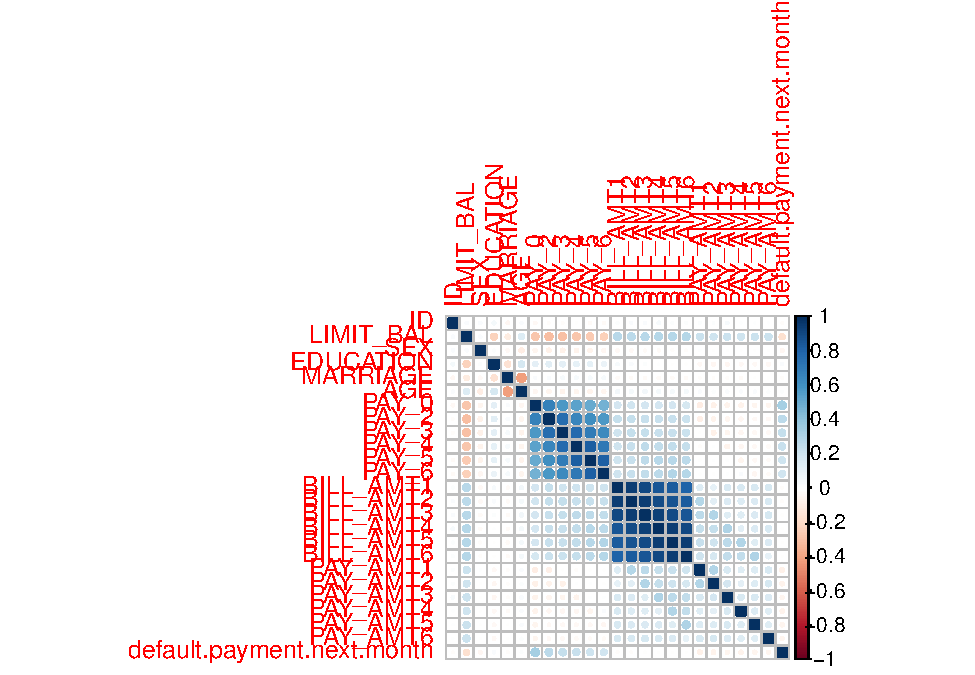
\includegraphics{assignment_q1_bmi_files/figure-latex/unnamed-chunk-8-1.pdf}

\begin{Shaded}
\begin{Highlighting}[]
\FunctionTok{plot}\NormalTok{(selected\_model)}
\end{Highlighting}
\end{Shaded}

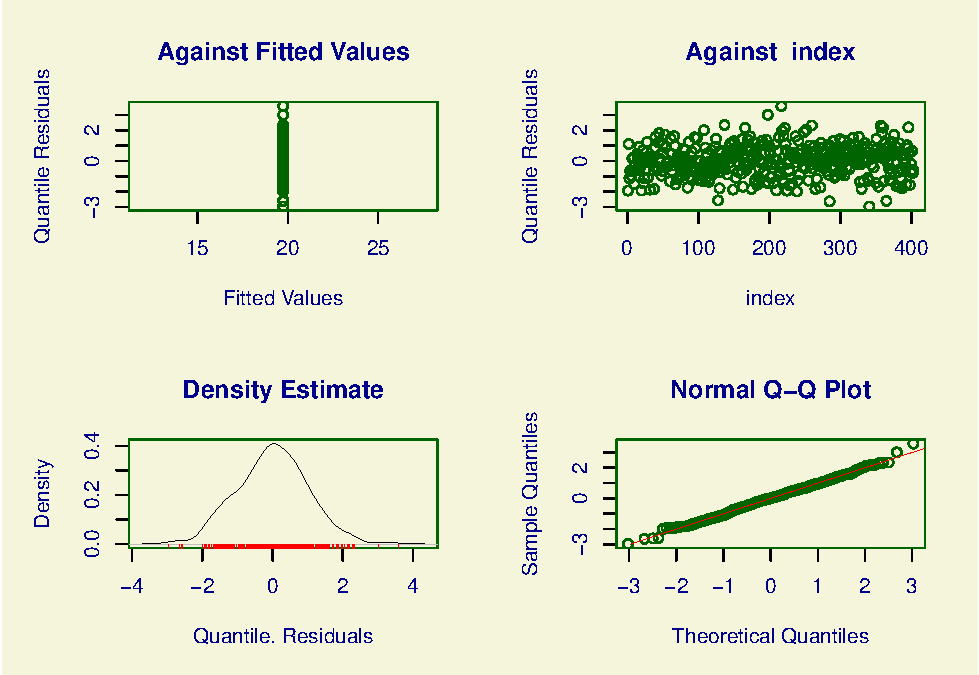
\includegraphics{assignment_q1_bmi_files/figure-latex/unnamed-chunk-8-2.pdf}

\begin{verbatim}
## ******************************************************************
##        Summary of the Quantile Residuals
##                            mean   =  1.028883e-06 
##                        variance   =  1.002488 
##                coef. of skewness  =  0.03768484 
##                coef. of kurtosis  =  3.121755 
## Filliben correlation coefficient  =  0.9983871 
## ******************************************************************
\end{verbatim}

The choice of distribution can be justified by comparing the Akaike
Information Criterion (AIC) values of the fitted models---the model with
the lowest AIC is typically preferred as it suggests a good fit with
relatively lower complexity.

\hypertarget{c-output-the-parameter-estimates-for-your-chosen-model}{%
\subsubsection{(c) Output the parameter estimates for your chosen
model}\label{c-output-the-parameter-estimates-for-your-chosen-model}}

Using the function summary() and interpret the fitted parameters. (You
may refer to the GAMLSS distribution book Rigby et al.~(2019) {[}2{]}
(or to its earlier version which can be found in the GAMLSS web-site
\url{https://www.gamlss.com}) to find what the distribution parameters
represent (i.e.~location, scale, kurtosis etc.).

Finally, for the chosen model, we can output the parameter estimates and
interpret them according to the distribution's characteristics.

\begin{Shaded}
\begin{Highlighting}[]
\CommentTok{\# Output parameter estimates for the chosen model}
\FunctionTok{summary}\NormalTok{(selected\_model)}
\end{Highlighting}
\end{Shaded}

\begin{verbatim}
## *******************************************************************
## Family:  c("JSU", "Johnson SU") 
## 
## Call:  gamlssML(formula = dbbmi_15$bmi, family = "JSU") 
## 
## Fitting method: "nlminb" 
## 
## 
## Coefficient(s):
##             Estimate  Std. Error   t value   Pr(>|t|)    
## eta.mu    19.7442002   0.1102768 179.04212 < 2.22e-16 ***
## eta.sigma  0.7952701   0.0534317  14.88385 < 2.22e-16 ***
## eta.nu     1.6219117   0.6555621   2.47408   0.013358 *  
## eta.tau    0.7379107   0.1869315   3.94749 7.8974e-05 ***
## ---
## Signif. codes:  0 '***' 0.001 '**' 0.01 '*' 0.05 '.' 0.1 ' ' 1
## 
##  Degrees of Freedom for the fit: 4 Residual Deg. of Freedom   399 
## Global Deviance:     1723.71 
##             AIC:     1731.71 
##             SBC:     1747.7
\end{verbatim}

\begin{Shaded}
\begin{Highlighting}[]
\FunctionTok{print}\NormalTok{(fit\_jsu}\SpecialCharTok{$}\NormalTok{mu.coefficients)}
\end{Highlighting}
\end{Shaded}

\begin{verbatim}
## (Intercept) 
##    19.74395
\end{verbatim}

Interpretation of the parameters will depend on the selected
distribution. For example:

\begin{itemize}
\item
  For a Normal distribution (\texttt{NO}), the parameters are the mean
  (\texttt{mu}) and standard deviation (\texttt{sigma}), representing
  the location and scale of the distribution.
\item
  For a Log-Normal distribution (\texttt{LOGNO}), \texttt{mu} and
  \texttt{sigma} represent the mean and standard deviation of the
  variable's logarithm, indicating the distribution's central tendency
  and spread on a log scale.
\item
  For a Gamma distribution (\texttt{GA}), the parameters might include a
  shape and a scale parameter, reflecting the distribution's skewness
  and scale.
\end{itemize}

Refer to the GAMLSS book or documentation for specific interpretations
of the parameters of your chosen distribution. The interpretation will
help in understanding the characteristics of BMI distribution among
Dutch boys aged 10 to 11, such as its central tendency, variability, and
potential skewness.

\begin{Shaded}
\begin{Highlighting}[]
\CommentTok{\# Function to calculate the fitted density}
\NormalTok{density\_fitted }\OtherTok{\textless{}{-}} \ControlFlowTok{function}\NormalTok{(x) \{}
  \FunctionTok{dJSU}\NormalTok{(x, }\AttributeTok{mu=}\NormalTok{fit\_jsu}\SpecialCharTok{$}\NormalTok{mu.coefficients, }\AttributeTok{sigma=}\NormalTok{fit\_jsu}\SpecialCharTok{$}\NormalTok{sigma.coefficients, }\AttributeTok{nu=}\NormalTok{fit\_jsu}\SpecialCharTok{$}\NormalTok{nu.coefficients, }\AttributeTok{tau=}\NormalTok{fit\_jsu}\SpecialCharTok{$}\NormalTok{tau.coefficients)}
\NormalTok{\}}

\CommentTok{\# Histogram with ggplot}
\NormalTok{p }\OtherTok{\textless{}{-}} \FunctionTok{ggplot}\NormalTok{(dbbmi\_15, }\FunctionTok{aes}\NormalTok{(}\AttributeTok{x=}\NormalTok{bmi15)) }\SpecialCharTok{+}
  \FunctionTok{geom\_histogram}\NormalTok{(}\FunctionTok{aes}\NormalTok{(}\AttributeTok{y=}\NormalTok{..density..), }\AttributeTok{binwidth =} \FloatTok{0.5}\NormalTok{, }\AttributeTok{colour=}\StringTok{"black"}\NormalTok{, }\AttributeTok{fill=}\StringTok{"white"}\NormalTok{) }

\CommentTok{\# Add the fitted model curve}
\NormalTok{p }\OtherTok{\textless{}{-}}\NormalTok{ p }\SpecialCharTok{+} \FunctionTok{stat\_function}\NormalTok{(}\AttributeTok{fun=}\NormalTok{density\_fitted, }\AttributeTok{colour=}\StringTok{"red"}\NormalTok{, }\AttributeTok{linewidth=}\DecValTok{1}\NormalTok{)}
\NormalTok{p}
\end{Highlighting}
\end{Shaded}

\includegraphics{assignment_q1_bmi_files/figure-latex/unnamed-chunk-10-1.pdf}
                   

\section{Appendix B: R Code for Question 3}

Analyse a different sample of 1000 from the original 3766
English boys. The data are stored in the packages \texttt{gamlss.data} under the
name grip and contain the variables grip and age. The aim here is to
create centile curves for grip given age.

\begin{Shaded}
\begin{Highlighting}[]
\CommentTok{\# Load the packages}
\FunctionTok{library}\NormalTok{(ggplot2)}
\FunctionTok{library}\NormalTok{(gamlss)}
\end{Highlighting}
\end{Shaded}

\begin{verbatim}
## Loading required package: splines
\end{verbatim}

\begin{verbatim}
## Loading required package: gamlss.data
\end{verbatim}

\begin{verbatim}
## 
## Attaching package: 'gamlss.data'
\end{verbatim}

\begin{verbatim}
## The following object is masked from 'package:datasets':
## 
##     sleep
\end{verbatim}

\begin{verbatim}
## Loading required package: gamlss.dist
\end{verbatim}

\begin{verbatim}
## Loading required package: nlme
\end{verbatim}

\begin{verbatim}
## Loading required package: parallel
\end{verbatim}

\begin{verbatim}
##  **********   GAMLSS Version 5.4-20  **********
\end{verbatim}

\begin{verbatim}
## For more on GAMLSS look at https://www.gamlss.com/
\end{verbatim}

\begin{verbatim}
## Type gamlssNews() to see new features/changes/bug fixes.
\end{verbatim}

\begin{Shaded}
\begin{Highlighting}[]
\FunctionTok{library}\NormalTok{(gamlss.ggplots)}
\end{Highlighting}
\end{Shaded}

\begin{verbatim}
## Loading required package: gamlss.foreach
\end{verbatim}

\begin{verbatim}
## Loading required package: foreach
\end{verbatim}

\begin{verbatim}
## Loading required package: doParallel
\end{verbatim}

\begin{verbatim}
## Loading required package: iterators
\end{verbatim}

\begin{Shaded}
\begin{Highlighting}[]
\FunctionTok{library}\NormalTok{(gamlss.add)}
\end{Highlighting}
\end{Shaded}

\begin{verbatim}
## Loading required package: mgcv
\end{verbatim}

\begin{verbatim}
## This is mgcv 1.9-0. For overview type 'help("mgcv-package")'.
\end{verbatim}

\begin{verbatim}
## Loading required package: nnet
\end{verbatim}

\begin{verbatim}
## 
## Attaching package: 'nnet'
\end{verbatim}

\begin{verbatim}
## The following object is masked from 'package:mgcv':
## 
##     multinom
\end{verbatim}

\begin{verbatim}
## Loading required package: rpart
\end{verbatim}

\begin{Shaded}
\begin{Highlighting}[]
\FunctionTok{library}\NormalTok{(gamlss.data)}
\end{Highlighting}
\end{Shaded}

Read the data file.

\begin{Shaded}
\begin{Highlighting}[]
\CommentTok{\# Load the data}
\FunctionTok{data}\NormalTok{(}\StringTok{"grip"}\NormalTok{, }\AttributeTok{package =} \StringTok{"gamlss.data"}\NormalTok{)}
\end{Highlighting}
\end{Shaded}

Set unique seed number, and select 1000 random rows.

\begin{Shaded}
\begin{Highlighting}[]
\FunctionTok{set.seed}\NormalTok{(}\DecValTok{567}\NormalTok{) }

\CommentTok{\# Sample 1000 observations}
\NormalTok{index }\OtherTok{\textless{}{-}} \FunctionTok{sample}\NormalTok{(}\FunctionTok{nrow}\NormalTok{(grip), }\DecValTok{1000}\NormalTok{)}
\NormalTok{grip\_sample }\OtherTok{\textless{}{-}}\NormalTok{ grip[index, ]}
\FunctionTok{dim}\NormalTok{(grip\_sample)}
\end{Highlighting}
\end{Shaded}

\begin{verbatim}
## [1] 1000    2
\end{verbatim}

Plot grip against age.

\begin{Shaded}
\begin{Highlighting}[]
\CommentTok{\# Plot grip against age}
\FunctionTok{plot}\NormalTok{(grip}\SpecialCharTok{$}\NormalTok{age, grip}\SpecialCharTok{$}\NormalTok{grip,}
     \AttributeTok{xlab =} \StringTok{"Age"}\NormalTok{,}
     \AttributeTok{ylab =} \StringTok{"Grip Strength"}\NormalTok{,}
     \AttributeTok{main =} \StringTok{"Grip Strength vs Age"}\NormalTok{,}
     \AttributeTok{col =} \StringTok{"blue"}\NormalTok{,}
     \AttributeTok{pch =} \DecValTok{19}\NormalTok{)}

\CommentTok{\# Add a smooth line to highlight the trend}
\FunctionTok{lines}\NormalTok{(}\FunctionTok{smooth.spline}\NormalTok{(grip}\SpecialCharTok{$}\NormalTok{age, grip}\SpecialCharTok{$}\NormalTok{grip), }\AttributeTok{col =} \StringTok{"red"}\NormalTok{)}
\end{Highlighting}
\end{Shaded}

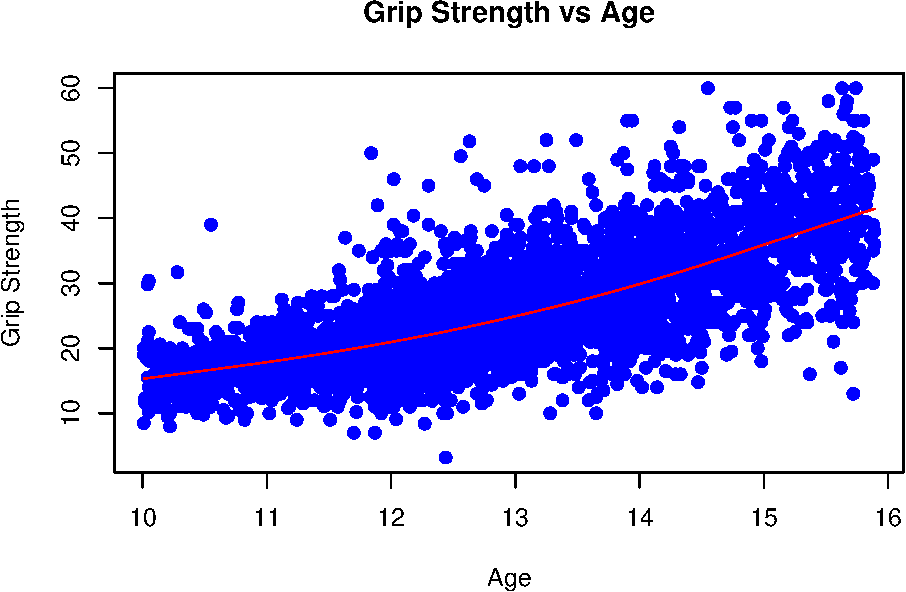
\includegraphics{assignment_q2_grip_files/figure-latex/unnamed-chunk-4-1.pdf}

\begin{Shaded}
\begin{Highlighting}[]
\CommentTok{\# Plot sample grip against age}
\FunctionTok{plot}\NormalTok{(grip\_sample}\SpecialCharTok{$}\NormalTok{age, grip\_sample}\SpecialCharTok{$}\NormalTok{grip,}
     \AttributeTok{xlab =} \StringTok{"Age"}\NormalTok{,}
     \AttributeTok{ylab =} \StringTok{"Grip Strength"}\NormalTok{,}
     \AttributeTok{main =} \StringTok{"Grip Strength vs Age"}\NormalTok{,}
     \AttributeTok{col =} \StringTok{"blue"}\NormalTok{,}
     \AttributeTok{pch =} \DecValTok{19}\NormalTok{)}

\CommentTok{\# Add a smooth line to highlight the trend}
\FunctionTok{lines}\NormalTok{(}\FunctionTok{smooth.spline}\NormalTok{(grip\_sample}\SpecialCharTok{$}\NormalTok{age, grip\_sample}\SpecialCharTok{$}\NormalTok{grip), }\AttributeTok{col =} \StringTok{"red"}\NormalTok{)}
\end{Highlighting}
\end{Shaded}

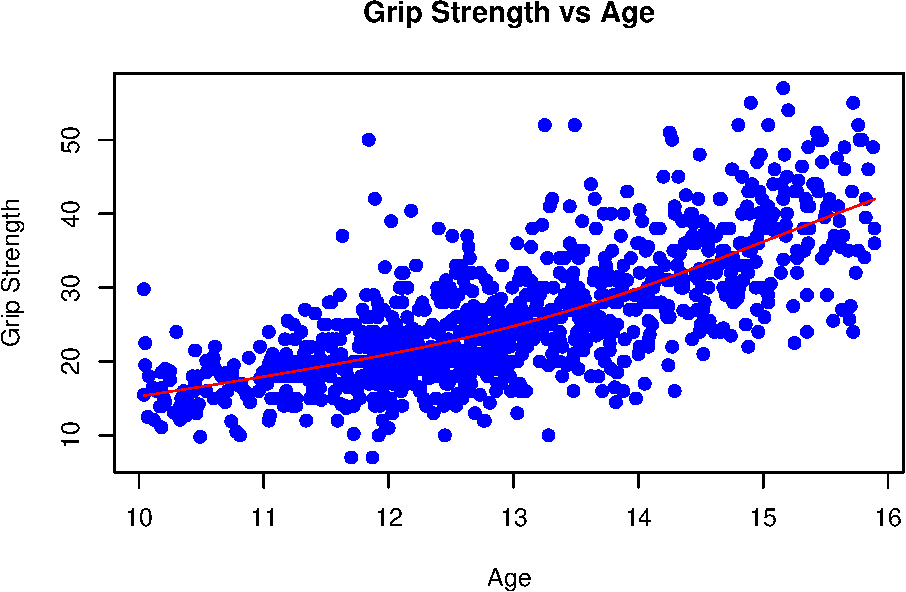
\includegraphics{assignment_q2_grip_files/figure-latex/unnamed-chunk-4-2.pdf}

Use the LMS method to fit the data.

\begin{Shaded}
\begin{Highlighting}[]
\CommentTok{\# Fit the model}
\NormalTok{gbccg }\OtherTok{\textless{}{-}} \FunctionTok{gamlss}\NormalTok{(grip }\SpecialCharTok{\textasciitilde{}} \FunctionTok{pb}\NormalTok{(age),}
                \AttributeTok{sigma.fo =} \SpecialCharTok{\textasciitilde{}} \FunctionTok{pb}\NormalTok{(age),}
                \AttributeTok{nu.fo =} \SpecialCharTok{\textasciitilde{}} \FunctionTok{pb}\NormalTok{(age),}
                \AttributeTok{data =}\NormalTok{ grip\_sample,}
                \AttributeTok{family =}\NormalTok{ BCCG)}
\end{Highlighting}
\end{Shaded}

\begin{verbatim}
## GAMLSS-RS iteration 1: Global Deviance = 6242.993 
## GAMLSS-RS iteration 2: Global Deviance = 6246.787 
## GAMLSS-RS iteration 3: Global Deviance = 6246.781 
## GAMLSS-RS iteration 4: Global Deviance = 6246.801 
## GAMLSS-RS iteration 5: Global Deviance = 6246.804 
## GAMLSS-RS iteration 6: Global Deviance = 6246.805
\end{verbatim}

\begin{Shaded}
\begin{Highlighting}[]
\CommentTok{\# Extract Effective Degrees of Freedom}
\NormalTok{edf\_details }\OtherTok{\textless{}{-}} \FunctionTok{edfAll}\NormalTok{(gbccg)}

\CommentTok{\# Print the EDF for each parameter}
\FunctionTok{print}\NormalTok{(edf\_details)}
\end{Highlighting}
\end{Shaded}

\begin{verbatim}
## $mu
## $mu$`pb(age)`
## [1] 4.713324
## 
## 
## $sigma
## $sigma$`pb(age)`
## [1] 3.319469
## 
## 
## $nu
## $nu$`pb(age)`
## [1] 2.000121
\end{verbatim}

Use the fitted values from the LMS model as starting values for fitting
the BCT and the BCPE distributions to the data

\begin{Shaded}
\begin{Highlighting}[]
\CommentTok{\# Fit the BCT model using gbccg as starting values}
\NormalTok{gbct }\OtherTok{\textless{}{-}} \FunctionTok{gamlss}\NormalTok{(grip }\SpecialCharTok{\textasciitilde{}} \FunctionTok{pb}\NormalTok{(age),}
               \AttributeTok{sigma.fo =} \SpecialCharTok{\textasciitilde{}} \FunctionTok{pb}\NormalTok{(age),}
               \AttributeTok{nu.fo =} \SpecialCharTok{\textasciitilde{}} \FunctionTok{pb}\NormalTok{(age),}
               \AttributeTok{tau.fo =} \SpecialCharTok{\textasciitilde{}} \FunctionTok{pb}\NormalTok{(age),}
               \AttributeTok{data =}\NormalTok{ grip\_sample,}
               \AttributeTok{family =}\NormalTok{ BCT,}
               \AttributeTok{start.from =}\NormalTok{ gbccg)}
\end{Highlighting}
\end{Shaded}

\begin{verbatim}
## GAMLSS-RS iteration 1: Global Deviance = 6243.64 
## GAMLSS-RS iteration 2: Global Deviance = 6241.875 
## GAMLSS-RS iteration 3: Global Deviance = 6241.464 
## GAMLSS-RS iteration 4: Global Deviance = 6241.311 
## GAMLSS-RS iteration 5: Global Deviance = 6241.251 
## GAMLSS-RS iteration 6: Global Deviance = 6241.225 
## GAMLSS-RS iteration 7: Global Deviance = 6241.215 
## GAMLSS-RS iteration 8: Global Deviance = 6241.208 
## GAMLSS-RS iteration 9: Global Deviance = 6241.206 
## GAMLSS-RS iteration 10: Global Deviance = 6241.205
\end{verbatim}

\begin{Shaded}
\begin{Highlighting}[]
\CommentTok{\# Fit the BCPE model using gbccg as starting values}
\NormalTok{gbcpe }\OtherTok{\textless{}{-}} \FunctionTok{gamlss}\NormalTok{(grip }\SpecialCharTok{\textasciitilde{}} \FunctionTok{pb}\NormalTok{(age),}
                \AttributeTok{sigma.fo =} \SpecialCharTok{\textasciitilde{}} \FunctionTok{pb}\NormalTok{(age),}
                \AttributeTok{nu.fo =} \SpecialCharTok{\textasciitilde{}} \FunctionTok{pb}\NormalTok{(age),}
                \AttributeTok{tau.fo =} \SpecialCharTok{\textasciitilde{}} \FunctionTok{pb}\NormalTok{(age),}
                \AttributeTok{data =}\NormalTok{ grip\_sample,}
                \AttributeTok{family =}\NormalTok{ BCPE,}
                \AttributeTok{start.from =}\NormalTok{ gbccg)}
\end{Highlighting}
\end{Shaded}

\begin{verbatim}
## GAMLSS-RS iteration 1: Global Deviance = 6241.603 
## GAMLSS-RS iteration 2: Global Deviance = 6241.32 
## GAMLSS-RS iteration 3: Global Deviance = 6241.293 
## GAMLSS-RS iteration 4: Global Deviance = 6241.292
\end{verbatim}

Effective degrees of freedom fitted for the parameters.

\begin{Shaded}
\begin{Highlighting}[]
\CommentTok{\# The EDF indicates the complexity of the model related to each parameter.}

\CommentTok{\# Extract EDF for BCT model}
\NormalTok{edf\_bct }\OtherTok{\textless{}{-}} \FunctionTok{edfAll}\NormalTok{(gbct)}

\CommentTok{\# Extract EDF for BCPE model}
\NormalTok{edf\_bcpe }\OtherTok{\textless{}{-}} \FunctionTok{edfAll}\NormalTok{(gbcpe)}

\CommentTok{\# Print the EDF for each model}
\FunctionTok{print}\NormalTok{(}\StringTok{"BCT EDF"}\NormalTok{)}
\end{Highlighting}
\end{Shaded}

\begin{verbatim}
## [1] "BCT EDF"
\end{verbatim}

\begin{Shaded}
\begin{Highlighting}[]
\FunctionTok{print}\NormalTok{(edf\_bct)}
\end{Highlighting}
\end{Shaded}

\begin{verbatim}
## $mu
## $mu$`pb(age)`
## [1] 4.733671
## 
## 
## $sigma
## $sigma$`pb(age)`
## [1] 3.444705
## 
## 
## $nu
## $nu$`pb(age)`
## [1] 2.000124
## 
## 
## $tau
## $tau$`pb(age)`
## [1] 2.000014
\end{verbatim}

\begin{Shaded}
\begin{Highlighting}[]
\FunctionTok{print}\NormalTok{(}\StringTok{"BCPE EDF"}\NormalTok{)}
\end{Highlighting}
\end{Shaded}

\begin{verbatim}
## [1] "BCPE EDF"
\end{verbatim}

\begin{Shaded}
\begin{Highlighting}[]
\FunctionTok{print}\NormalTok{(edf\_bcpe)}
\end{Highlighting}
\end{Shaded}

\begin{verbatim}
## $mu
## $mu$`pb(age)`
## [1] 4.727011
## 
## 
## $sigma
## $sigma$`pb(age)`
## [1] 3.350044
## 
## 
## $nu
## $nu$`pb(age)`
## [1] 2.000108
## 
## 
## $tau
## $tau$`pb(age)`
## [1] 2.000317
\end{verbatim}

\begin{Shaded}
\begin{Highlighting}[]
\FunctionTok{edfAll}\NormalTok{(gbcpe)}
\end{Highlighting}
\end{Shaded}

\begin{verbatim}
## $mu
## $mu$`pb(age)`
## [1] 4.727011
## 
## 
## $sigma
## $sigma$`pb(age)`
## [1] 3.350044
## 
## 
## $nu
## $nu$`pb(age)`
## [1] 2.000108
## 
## 
## $tau
## $tau$`pb(age)`
## [1] 2.000317
\end{verbatim}

GAIC to compare the three models.

\begin{Shaded}
\begin{Highlighting}[]
\CommentTok{\# Calculate GAIC for each model}
\NormalTok{gaic\_bccg }\OtherTok{\textless{}{-}} \FunctionTok{GAIC}\NormalTok{(gbccg)}
\NormalTok{gaic\_gbct }\OtherTok{\textless{}{-}} \FunctionTok{GAIC}\NormalTok{(gbct)}
\NormalTok{gaic\_gbcpe }\OtherTok{\textless{}{-}} \FunctionTok{GAIC}\NormalTok{(gbcpe)}

\CommentTok{\# Print the GAIC values}
\FunctionTok{print}\NormalTok{(}\FunctionTok{paste}\NormalTok{(}\StringTok{"GAIC for BCCG:"}\NormalTok{, gaic\_bccg))}
\end{Highlighting}
\end{Shaded}

\begin{verbatim}
## [1] "GAIC for BCCG: 6266.87079383024"
\end{verbatim}

\begin{Shaded}
\begin{Highlighting}[]
\FunctionTok{print}\NormalTok{(}\FunctionTok{paste}\NormalTok{(}\StringTok{"GAIC for BCT:"}\NormalTok{, gaic\_gbct))}
\end{Highlighting}
\end{Shaded}

\begin{verbatim}
## [1] "GAIC for BCT: 6265.56229903994"
\end{verbatim}

\begin{Shaded}
\begin{Highlighting}[]
\FunctionTok{print}\NormalTok{(}\FunctionTok{paste}\NormalTok{(}\StringTok{"GAIC for BCPE:"}\NormalTok{, gaic\_gbcpe))}
\end{Highlighting}
\end{Shaded}

\begin{verbatim}
## [1] "GAIC for BCPE: 6265.44681092804"
\end{verbatim}

Plot the fitted parameters for the fitted models in (d) and (e) using
for example

\begin{Shaded}
\begin{Highlighting}[]
\CommentTok{\# Assuming \textquotesingle{}grip\_sample\textquotesingle{} is your dataset and \textquotesingle{}gbccg\textquotesingle{} and \textquotesingle{}gbct\textquotesingle{} are fitted models}
\FunctionTok{fittedPlot}\NormalTok{(gbccg, gbct, }\AttributeTok{x=}\NormalTok{grip\_sample}\SpecialCharTok{$}\NormalTok{age)}
\end{Highlighting}
\end{Shaded}

\includegraphics{assignment_q2_grip_files/figure-latex/unnamed-chunk-10-1.pdf}

\begin{Shaded}
\begin{Highlighting}[]
\CommentTok{\# Calculate fitted values or centiles for each model across a range of ages}
\NormalTok{age\_seq }\OtherTok{\textless{}{-}} \FunctionTok{seq}\NormalTok{(}\FunctionTok{min}\NormalTok{(grip\_sample}\SpecialCharTok{$}\NormalTok{age), }\FunctionTok{max}\NormalTok{(grip\_sample}\SpecialCharTok{$}\NormalTok{age), }\AttributeTok{length.out =} \DecValTok{100}\NormalTok{)}

\CommentTok{\# For BCCG Model}
\NormalTok{fitted\_bccg }\OtherTok{\textless{}{-}} \FunctionTok{predict}\NormalTok{(gbccg, }\AttributeTok{newdata=}\FunctionTok{data.frame}\NormalTok{(}\AttributeTok{age=}\NormalTok{age\_seq), }\AttributeTok{type=}\StringTok{"response"}\NormalTok{)}
\end{Highlighting}
\end{Shaded}

\begin{verbatim}
## new prediction
\end{verbatim}

\begin{Shaded}
\begin{Highlighting}[]
\CommentTok{\# For BCT Model}
\NormalTok{fitted\_gbct }\OtherTok{\textless{}{-}} \FunctionTok{predict}\NormalTok{(gbct, }\AttributeTok{newdata=}\FunctionTok{data.frame}\NormalTok{(}\AttributeTok{age=}\NormalTok{age\_seq), }\AttributeTok{type=}\StringTok{"response"}\NormalTok{)}
\end{Highlighting}
\end{Shaded}

\begin{verbatim}
## new prediction
\end{verbatim}

\begin{Shaded}
\begin{Highlighting}[]
\CommentTok{\# Plotting}
\FunctionTok{plot}\NormalTok{(age\_seq, fitted\_bccg, }\AttributeTok{type=}\StringTok{\textquotesingle{}l\textquotesingle{}}\NormalTok{, }\AttributeTok{col=}\StringTok{\textquotesingle{}blue\textquotesingle{}}\NormalTok{, }\AttributeTok{ylim=}\FunctionTok{range}\NormalTok{(}\FunctionTok{c}\NormalTok{(fitted\_bccg, fitted\_gbct)),}
     \AttributeTok{xlab=}\StringTok{\textquotesingle{}Age\textquotesingle{}}\NormalTok{, }\AttributeTok{ylab=}\StringTok{\textquotesingle{}Fitted Grip Strength\textquotesingle{}}\NormalTok{, }\AttributeTok{main=}\StringTok{\textquotesingle{}Fitted Models Comparison\textquotesingle{}}\NormalTok{)}
\FunctionTok{lines}\NormalTok{(age\_seq, fitted\_gbct, }\AttributeTok{col=}\StringTok{\textquotesingle{}red\textquotesingle{}}\NormalTok{)}

\CommentTok{\# Adding a legend}
\FunctionTok{legend}\NormalTok{(}\StringTok{"topright"}\NormalTok{, }\AttributeTok{legend=}\FunctionTok{c}\NormalTok{(}\StringTok{"BCCG"}\NormalTok{, }\StringTok{"BCT"}\NormalTok{), }\AttributeTok{col=}\FunctionTok{c}\NormalTok{(}\StringTok{"blue"}\NormalTok{, }\StringTok{"red"}\NormalTok{), }\AttributeTok{lty=}\DecValTok{1}\NormalTok{, }\AttributeTok{cex=}\FloatTok{0.8}\NormalTok{)}
\end{Highlighting}
\end{Shaded}

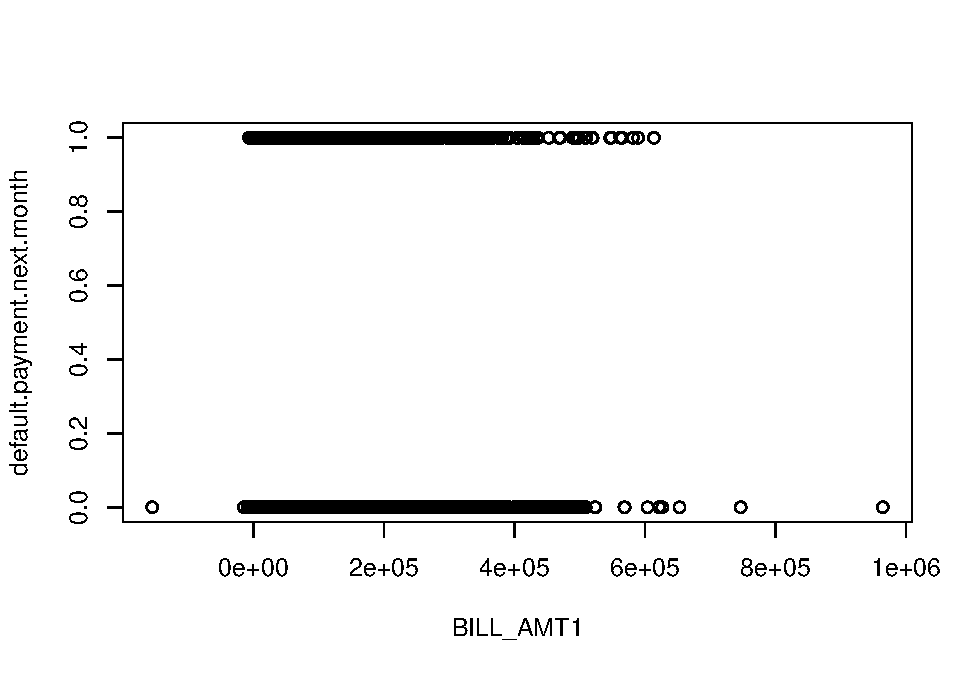
\includegraphics{assignment_q2_grip_files/figure-latex/unnamed-chunk-10-2.pdf}

Centile plot for the fitted models.

\begin{Shaded}
\begin{Highlighting}[]
\FunctionTok{centilesTwo}\NormalTok{(gbccg, }\DecValTok{10}\SpecialCharTok{:}\DecValTok{16}\NormalTok{, }\FunctionTok{seq}\NormalTok{(}\DecValTok{15}\NormalTok{, }\DecValTok{40}\NormalTok{, }\DecValTok{5}\NormalTok{), age,  grip, }\AttributeTok{cent=}\FloatTok{0.05}\NormalTok{, }\AttributeTok{dist=}\NormalTok{.}\DecValTok{1}\NormalTok{, }\AttributeTok{xlab=}\StringTok{"age"}\NormalTok{, }\AttributeTok{ylab=}\StringTok{\textquotesingle{}grip\textquotesingle{}}\NormalTok{)}
\end{Highlighting}
\end{Shaded}

\begin{verbatim}
## new prediction 
## new prediction 
## new prediction
\end{verbatim}

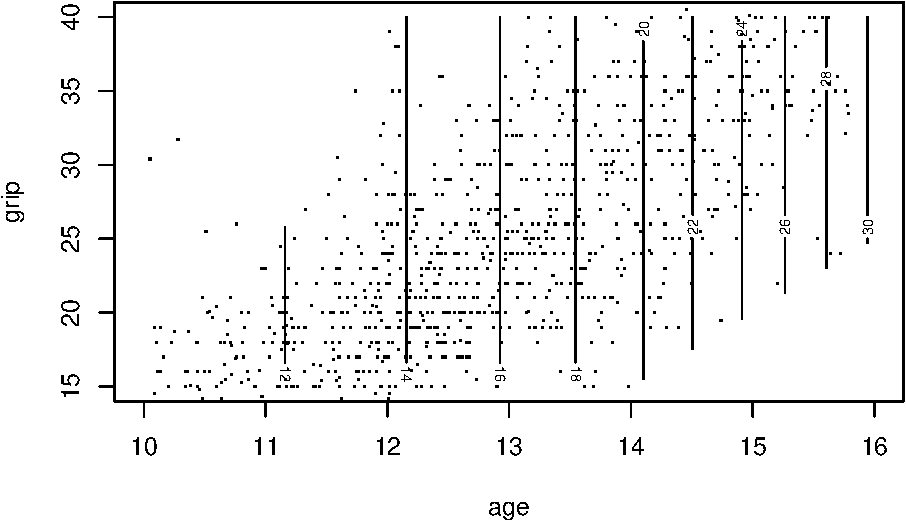
\includegraphics{assignment_q2_grip_files/figure-latex/unnamed-chunk-11-1.pdf}

\begin{Shaded}
\begin{Highlighting}[]
\FunctionTok{centiles}\NormalTok{(gbccg, }\AttributeTok{xvar=}\NormalTok{grip\_sample}\SpecialCharTok{$}\NormalTok{age, }\AttributeTok{cent=}\FunctionTok{c}\NormalTok{(}\FloatTok{0.1}\NormalTok{, }\FloatTok{0.4}\NormalTok{, }\DecValTok{2}\NormalTok{,}\DecValTok{10}\NormalTok{, }\DecValTok{25}\NormalTok{, }\DecValTok{50}\NormalTok{,}\DecValTok{75}\NormalTok{,}\DecValTok{90}\NormalTok{,}\DecValTok{98}\NormalTok{,}\FloatTok{99.6}\NormalTok{, }\FloatTok{99.9}\NormalTok{), }\AttributeTok{ylab=}\StringTok{"grip"}\NormalTok{, }\AttributeTok{xlab=}\StringTok{"age"}\NormalTok{, }\AttributeTok{legend=}\ConstantTok{FALSE}\NormalTok{)}
\end{Highlighting}
\end{Shaded}

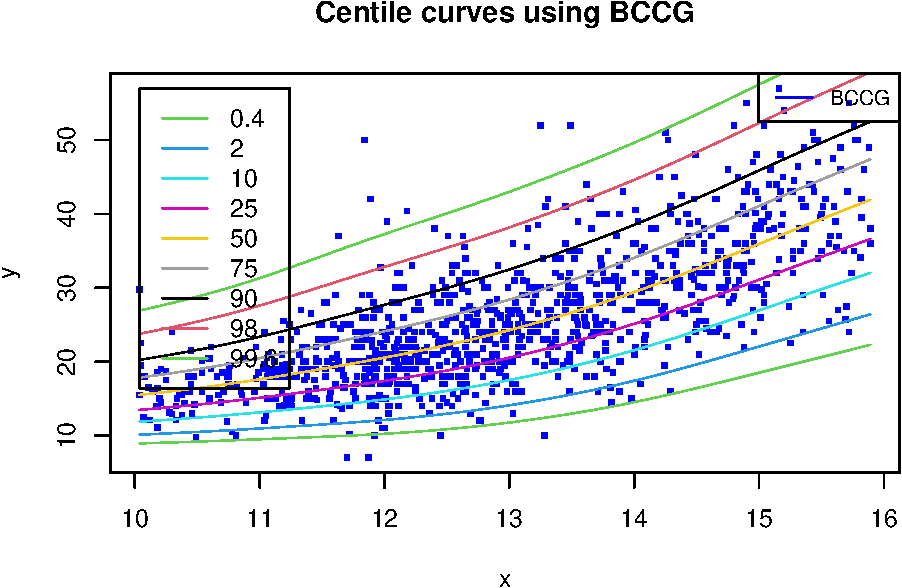
\includegraphics{assignment_q2_grip_files/figure-latex/unnamed-chunk-11-2.pdf}

\begin{verbatim}
## % of cases below  0.1 centile is  0.2 
## % of cases below  0.4 centile is  0.7 
## % of cases below  2 centile is  2.3 
## % of cases below  10 centile is  8.7 
## % of cases below  25 centile is  24.8 
## % of cases below  50 centile is  49.9 
## % of cases below  75 centile is  75 
## % of cases below  90 centile is  91.2 
## % of cases below  98 centile is  97.9 
## % of cases below  99.6 centile is  99.1 
## % of cases below  99.9 centile is  99.7
\end{verbatim}

\begin{Shaded}
\begin{Highlighting}[]
\CommentTok{\# Plot centiles for BCCG model}
\FunctionTok{plot}\NormalTok{(grip\_sample}\SpecialCharTok{$}\NormalTok{age, grip\_sample}\SpecialCharTok{$}\NormalTok{grip, }\AttributeTok{col=}\StringTok{"gray90"}\NormalTok{, }\AttributeTok{main=}\StringTok{"Centile Comparison"}\NormalTok{, }\AttributeTok{xlab=}\StringTok{"Age"}\NormalTok{, }\AttributeTok{ylab=}\StringTok{"Grip Strength"}\NormalTok{)}
\end{Highlighting}
\end{Shaded}

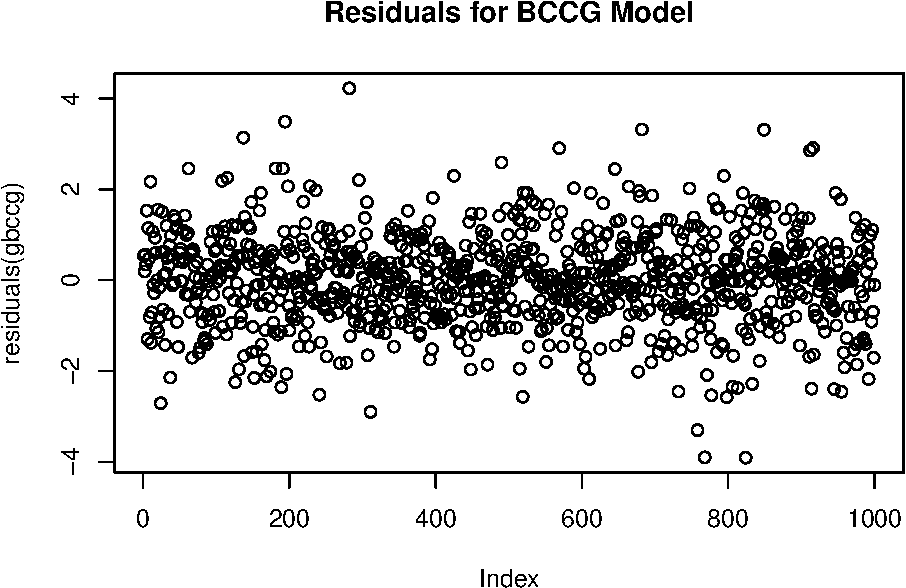
\includegraphics{assignment_q2_grip_files/figure-latex/unnamed-chunk-12-1.pdf}

\begin{Shaded}
\begin{Highlighting}[]
\FunctionTok{centiles}\NormalTok{(gbccg, }\AttributeTok{xvar =}\NormalTok{ grip\_sample}\SpecialCharTok{$}\NormalTok{age, }\AttributeTok{col =} \StringTok{"blue"}\NormalTok{, }\AttributeTok{lty =} \DecValTok{1}\NormalTok{) }\CommentTok{\#, add = TRUE}
\end{Highlighting}
\end{Shaded}

\begin{verbatim}
## % of cases below  0.4 centile is  0.7 
## % of cases below  2 centile is  2.3 
## % of cases below  10 centile is  8.7 
## % of cases below  25 centile is  24.8 
## % of cases below  50 centile is  49.9 
## % of cases below  75 centile is  75 
## % of cases below  90 centile is  91.2 
## % of cases below  98 centile is  97.9 
## % of cases below  99.6 centile is  99.1
\end{verbatim}

\begin{Shaded}
\begin{Highlighting}[]
\FunctionTok{legend}\NormalTok{(}\StringTok{"topright"}\NormalTok{, }\AttributeTok{legend=}\FunctionTok{c}\NormalTok{(}\StringTok{"BCCG"}\NormalTok{), }\AttributeTok{col=}\FunctionTok{c}\NormalTok{(}\StringTok{"blue"}\NormalTok{), }\AttributeTok{lty=}\DecValTok{1}\NormalTok{, }\AttributeTok{cex=}\FloatTok{0.8}\NormalTok{)}
\end{Highlighting}
\end{Shaded}

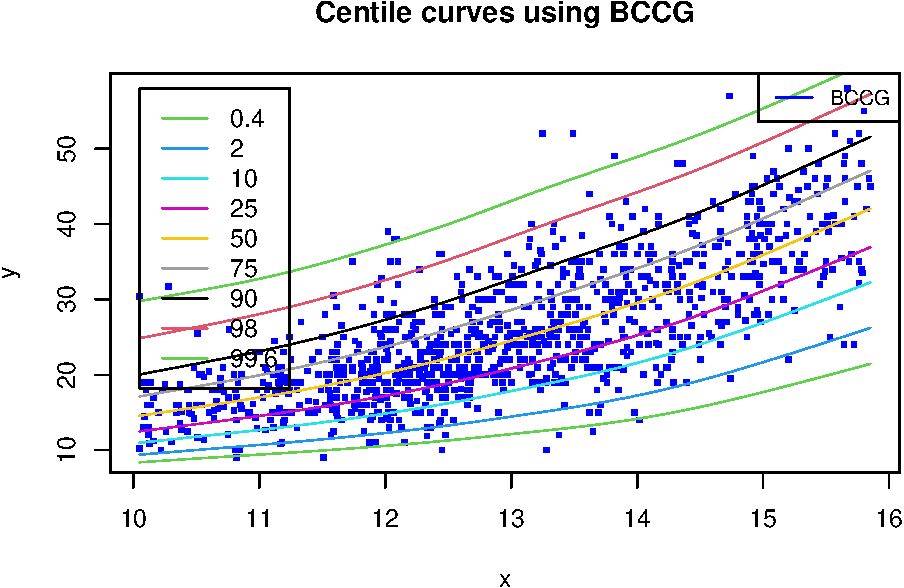
\includegraphics{assignment_q2_grip_files/figure-latex/unnamed-chunk-12-2.pdf}

\begin{Shaded}
\begin{Highlighting}[]
\CommentTok{\# Add centiles for BCT model to the existing plot}
\FunctionTok{centiles}\NormalTok{(gbct, }\AttributeTok{xvar =}\NormalTok{ grip\_sample}\SpecialCharTok{$}\NormalTok{age, }\AttributeTok{col =} \StringTok{"blue"}\NormalTok{, }\AttributeTok{lty =} \DecValTok{2}\NormalTok{)}
\end{Highlighting}
\end{Shaded}

\begin{verbatim}
## % of cases below  0.4 centile is  0.5 
## % of cases below  2 centile is  2.3 
## % of cases below  10 centile is  9.3 
## % of cases below  25 centile is  25.3 
## % of cases below  50 centile is  50 
## % of cases below  75 centile is  74.4 
## % of cases below  90 centile is  90.4 
## % of cases below  98 centile is  98 
## % of cases below  99.6 centile is  99.6
\end{verbatim}

\begin{Shaded}
\begin{Highlighting}[]
\CommentTok{\# Update the legend to include BCT}
\FunctionTok{legend}\NormalTok{(}\StringTok{"topright"}\NormalTok{, }\AttributeTok{legend=}\FunctionTok{c}\NormalTok{(}\StringTok{"BCT"}\NormalTok{), }\AttributeTok{col=}\FunctionTok{c}\NormalTok{(}\StringTok{"blue"}\NormalTok{), }\AttributeTok{lty=}\DecValTok{1}\SpecialCharTok{:}\DecValTok{2}\NormalTok{, }\AttributeTok{cex=}\FloatTok{0.8}\NormalTok{)}
\end{Highlighting}
\end{Shaded}

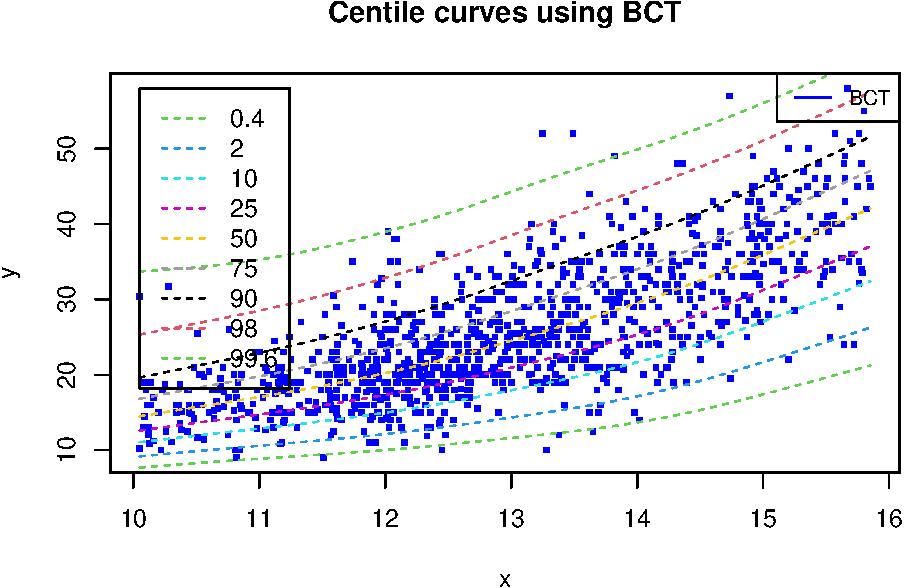
\includegraphics{assignment_q2_grip_files/figure-latex/unnamed-chunk-12-3.pdf}

Residuals from the fitted models:

\begin{Shaded}
\begin{Highlighting}[]
\CommentTok{\# For BCCG Model}
\FunctionTok{plot}\NormalTok{(}\FunctionTok{residuals}\NormalTok{(gbccg), }\AttributeTok{main=}\StringTok{"Residuals for BCCG Model"}\NormalTok{)}
\end{Highlighting}
\end{Shaded}

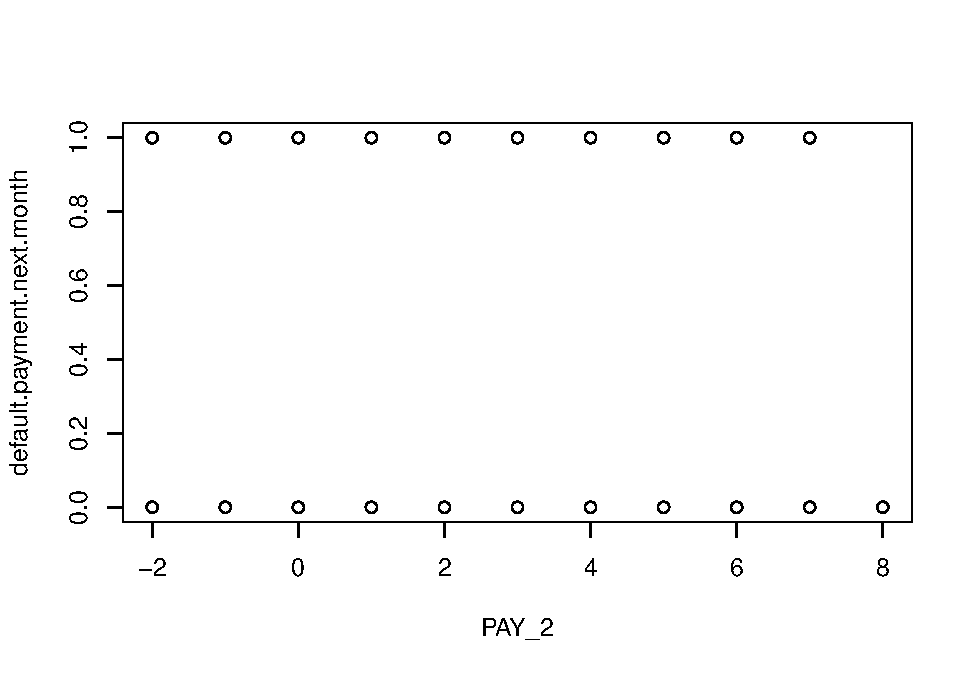
\includegraphics{assignment_q2_grip_files/figure-latex/unnamed-chunk-13-1.pdf}

\begin{Shaded}
\begin{Highlighting}[]
\CommentTok{\# For BCT Model}
\FunctionTok{plot}\NormalTok{(}\FunctionTok{residuals}\NormalTok{(gbct), }\AttributeTok{main=}\StringTok{"Residuals for BCT Model"}\NormalTok{)}
\end{Highlighting}
\end{Shaded}

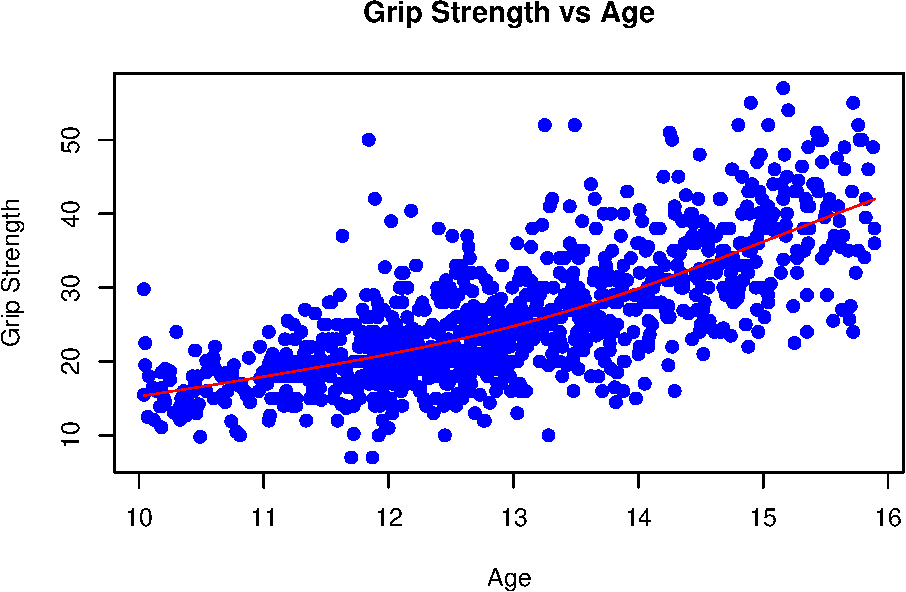
\includegraphics{assignment_q2_grip_files/figure-latex/unnamed-chunk-13-2.pdf}

\begin{Shaded}
\begin{Highlighting}[]
\CommentTok{\# For BCCG Model}
\FunctionTok{wp}\NormalTok{(gbccg, }\AttributeTok{main=}\StringTok{"Worm Plot for BCCG Model"}\NormalTok{)}
\end{Highlighting}
\end{Shaded}

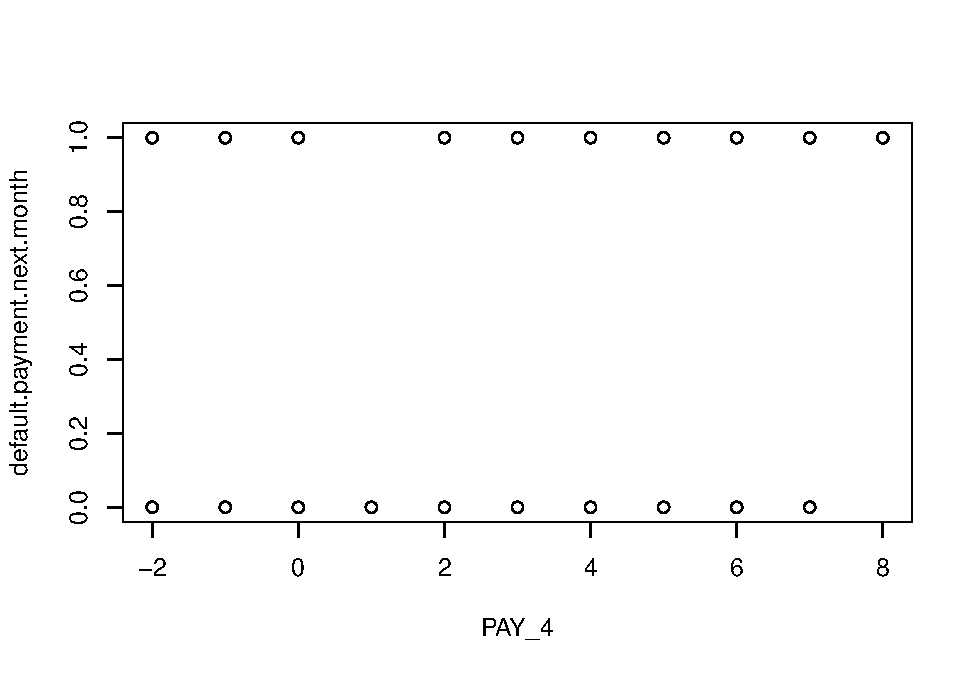
\includegraphics{assignment_q2_grip_files/figure-latex/unnamed-chunk-13-3.pdf}

\begin{Shaded}
\begin{Highlighting}[]
\CommentTok{\# For BCT Model}
\FunctionTok{wp}\NormalTok{(gbct, }\AttributeTok{main=}\StringTok{"Worm Plot for BCT Model"}\NormalTok{)}
\end{Highlighting}
\end{Shaded}

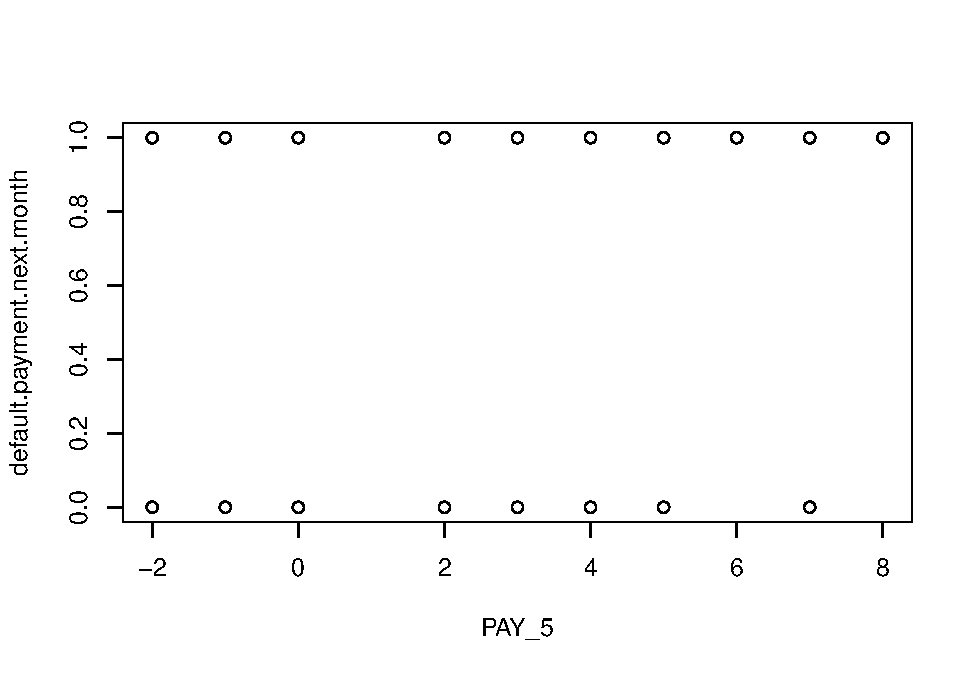
\includegraphics{assignment_q2_grip_files/figure-latex/unnamed-chunk-13-4.pdf}

\begin{Shaded}
\begin{Highlighting}[]
\CommentTok{\# For BCCG Model}
\NormalTok{qstats\_bccg }\OtherTok{\textless{}{-}} \FunctionTok{Q.stats}\NormalTok{(gbccg)}
\end{Highlighting}
\end{Shaded}

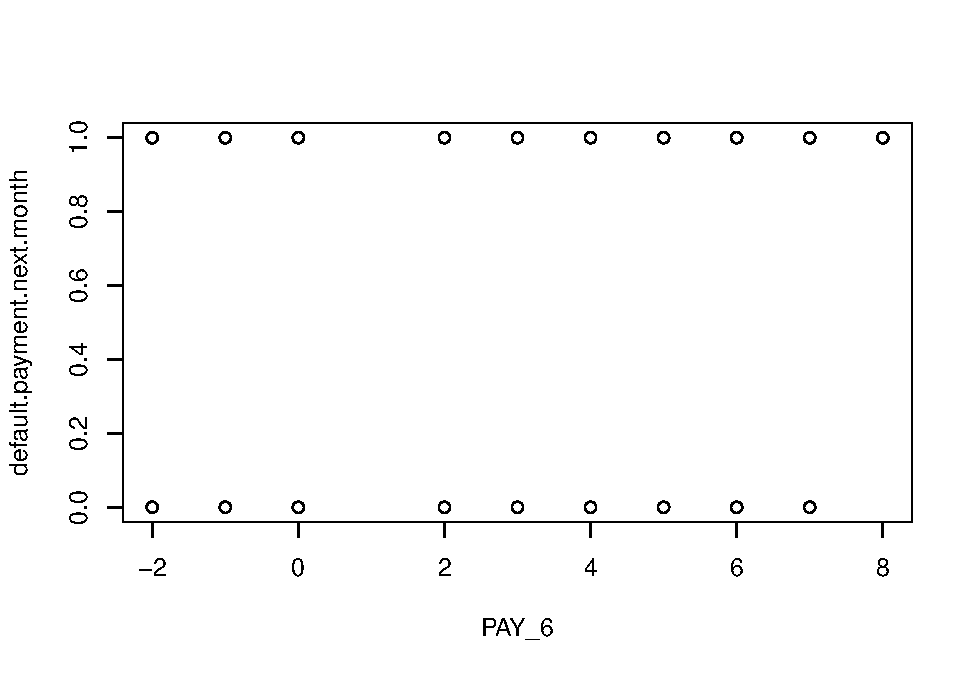
\includegraphics{assignment_q2_grip_files/figure-latex/unnamed-chunk-13-5.pdf}

\begin{Shaded}
\begin{Highlighting}[]
\FunctionTok{print}\NormalTok{(qstats\_bccg)}
\end{Highlighting}
\end{Shaded}

\begin{verbatim}
##                             Z1          Z2          Z3          Z4   AgostinoK2
##    0.5 to  100.5  -0.203907433  1.85395837 -1.96268227  0.75852485  4.427481630
##  100.5 to  200.5   2.402287804  0.28062802 -0.85776506 -2.79366506  8.540325397
##  200.5 to  300.5   0.871410159 -1.19936605  1.04028580  1.20345279  2.530493158
##  300.5 to  400.5   0.215184771 -1.49021285  1.85291013  2.70760397 10.764395207
##  400.5 to  500.5  -1.531442363 -2.15310227 -0.41383582  1.19895473  1.608752543
##  500.5 to  600.5   0.037281474 -0.06330455  0.56132156  0.86459185  1.062600958
##  600.5 to  700.5   0.416330909  1.38978751 -0.16687341  0.62308483  0.416081434
##  700.5 to  800.5  -0.930585700  0.51356221  1.05915525  1.26446329  2.720677240
##  800.5 to  900.5  -1.306755289  0.99110231  0.31603114  1.05594507  1.214895675
##  900.5 to 1000.5  -0.005296923 -1.25765363  0.08189189 -0.04731519  0.008945009
## TOTAL Q stats     11.711889316 16.57421573 10.84593361 22.44871464 33.294648249
## df for Q stats     5.286675988  7.84026565  7.99987911 10.00000000 17.999879110
## p-val for Q stats  0.046334806  0.03214421  0.21057399  0.01297493  0.015370373
##                      N
##    0.5 to  100.5   100
##  100.5 to  200.5   100
##  200.5 to  300.5   100
##  300.5 to  400.5   100
##  400.5 to  500.5   100
##  500.5 to  600.5   100
##  600.5 to  700.5   100
##  700.5 to  800.5   100
##  800.5 to  900.5   100
##  900.5 to 1000.5   100
## TOTAL Q stats     1000
## df for Q stats       0
## p-val for Q stats    0
\end{verbatim}

\begin{Shaded}
\begin{Highlighting}[]
\CommentTok{\# For BCT Model}
\NormalTok{qstats\_bct }\OtherTok{\textless{}{-}} \FunctionTok{Q.stats}\NormalTok{(gbct)}
\end{Highlighting}
\end{Shaded}

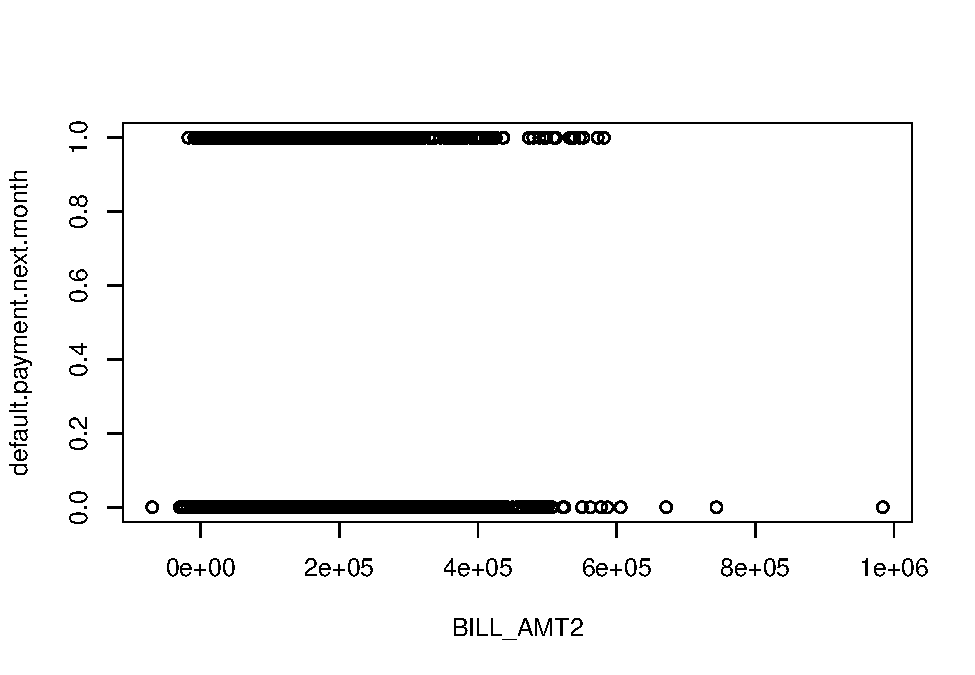
\includegraphics{assignment_q2_grip_files/figure-latex/unnamed-chunk-13-6.pdf}

\begin{Shaded}
\begin{Highlighting}[]
\FunctionTok{print}\NormalTok{(qstats\_bct)}
\end{Highlighting}
\end{Shaded}

\begin{verbatim}
##                             Z1          Z2         Z3          Z4  AgostinoK2
##    0.5 to  100.5  -0.150324437  1.75960447 -1.6292108  0.11704128  2.66802637
##  100.5 to  200.5   2.440492979  0.46954000 -0.9804560 -3.29497276 11.81813938
##  200.5 to  300.5   0.842962204 -1.08562505  0.5829998  0.33028150  0.44897466
##  300.5 to  400.5   0.170958501 -1.54178728  1.3770034  2.20209601  6.74536534
##  400.5 to  500.5  -1.523487794 -2.03988375  0.1163577  0.18062149  0.04616323
##  500.5 to  600.5   0.008605278 -0.02454827  0.3727182  0.31449406  0.23782540
##  600.5 to  700.5   0.440857942  1.23288881 -0.1201984  0.04439974  0.01641898
##  700.5 to  800.5  -0.937084732  0.46479961  0.8224300  0.44323903  0.87285192
##  800.5 to  900.5  -1.325056094  0.82985742  0.2824048  0.30526034  0.17293634
##  900.5 to 1000.5  -0.019382405 -1.11202793  0.0777290 -0.47198845  0.22881489
## TOTAL Q stats     11.868137464 14.69541676  6.7807399 16.47477665 23.25551652
## df for Q stats     5.266329280  7.77764748  7.9998764  7.99998585 15.99986227
## p-val for Q stats  0.043121921  0.05898312  0.5604506  0.03606707  0.10706852
##                      N
##    0.5 to  100.5   100
##  100.5 to  200.5   100
##  200.5 to  300.5   100
##  300.5 to  400.5   100
##  400.5 to  500.5   100
##  500.5 to  600.5   100
##  600.5 to  700.5   100
##  700.5 to  800.5   100
##  800.5 to  900.5   100
##  900.5 to 1000.5   100
## TOTAL Q stats     1000
## df for Q stats       0
## p-val for Q stats    0
\end{verbatim}
                   

\section{Appendix C: R Code for Question 3}

%\section{Appendix: Full R Code}

Description of implementation, etc
 
\subsection{Q1 R Code}

\begin{listing}[!ht]
\inputminted{R}{./tex/code/assignment1.r}
\caption{R Q1 code}
\label{listing:1}
\end{listing}

\subsection{Q2 R Code}

\subsection{Q3 R Code}

                   

\end{document}

%%% Local Variables:
%%% mode: latex
%%% TeX-master: t
%%% End:
